

\newcommand{\BF}{\mathbf{F}}
\newcommand{\BZ}{\mathbf{Z}}
\newcommand{\BA}{\mathbf{A}}
\newcommand{\BB}{\mathbf{B}}
\newcommand{\BC}{\mathbf{C}}
\newcommand{\BD}{\mathbf{D}}

The major role of this work is to explore the mechanism which helps humans to learn the compliant force dynamics. This would enable us to get an in-depth understanding of how humans modulate their whole-body motion to reach anticipated goals ruled by the external force. Further, this would be beneficial to apply it for controlling the humanoid robot in order to keep a stable posture when interacting with multiple compliant surfaces. 

With reference to the results of the pilot experiment (see the D2.2), the experimental design has been developed and further human subject experiments were conducted to examine the human learnability factor in different force dynamics. Three different types of forces (simple linear and two non-linear forces) were generated and the human movements to reach the anticipated goal were measured against the compliant forces.
%%%%%%%%%%%%%%%%%%%%%%%%%%%%%%%%%%%%%%%%%%%%%%%%%%%%%%%%%%%%%%%%%%%%%%%%%%%%%%%%
\subsection{Introduction}

Studying human strategies of dealing with uncertain contact is important to formulate equivalent humanoid robot behaviour, in particular with multiple non-rigid contacts. In the real-world interactions, there are varied and complicated force dynamics (i.e., governed by not only simple linear principles) when making a contact with an object and handling it. Humans can learn a new force dynamics through sensorimotor learning and adaptation, and they can control their whole body movements to the desired contact in an uncertain environment. The CNS (Central Nervous System) seems to generalise the dynamics through visuomotor learning, and the formalisation enables humans to predict the consequence of action and to achieve the behavioural goal optimally \cite{Wolpert2011, Davidson2003}. Previous studies have shown that a certain exposure (repetitive movements) against forces facilitates to learn the spatial and temporal characteristics of the interaction via error-based visuomotor perturbation paradigm \cite{Goodbody1998, Krakuer2006}. Humans likely generalize the force principles in a cognitively robust way and optimise their body movements interacting with the force. However, the detailed process and the underlying mechanisms are little unknown.

Like humans, robots are required to flexibly adjust their posture and coordinate the physical mobility with augmented autonomy. The CoDyCo project has been investigating the humanoid robot’s whole-body coordination mechanisms in arm reaching movements and the postural balance control in assistive contact with rigid and/or compliant surfaces \cite{Azad2015}. In the project, aiming to devise robot balance control optimally, we need a deeper insight into how humans perform with a novel environment and how quickly they establish stable body posture and supporting contacts. The successful modelling in humans could directly apply for the autonomous whole-body balance control in interacting with the environment through supportive contacts.

In the previous pilot experiment, which was reported in the D2.2, we examined human behaviour on learning compliant contacts. Participants were asked to push a robot arm to reach a certain target position against a compliant surface with a simple linear force, generated by a haptic device. After the learning session with a certain time period, we probed the participants’ behaviour to reach the double distance from the learning session with the same force dynamics as a test trial. The results showed that most participants reached the test target position much faster than the expectation based on the distance. This seems to indicate that participants did not well employ the principle to reach the new anticipated goal; rather they might have followed their own rule.

Based on these pilot study results, we speculate if participants might have learned the timing through the repetitive movements at the learning session and they have maintained their own rhythms to reach the anticipated goal. Several studies indicated that time perception plays an important role in human motor control \cite{Berret2016, Goodbody1998, Rank2015}. Therefore, we considered to modify the experimental design to prevent participants regulate their own rhythms for the task. In the current experiment, we set a certain time windows to reach the target at the learning block but removed the consecutive evaluation in order to avoid the excessive exposure before probing their anticipated goal-directed behaviour. We also minimised the visual information as much as possible in the task, considering the effect on the human force perception as well.

The current study helps in exploring and solving the following research questions: 1. Do humans learn and understand different forces applied in their daily activity? 2. How do they differentiate between linear and non-linear forces perceptually? ”. In the experiment, developed from the previous pilot experiment, we generated three different types of forces and measured the motor control performance against the forces and examined the human learnability of different force dynamics. Since, human-haptic perception is subjective to the force applied, contact force and the compliance of the system \cite{van2014}; we introduced a questionnaire to evaluate their perceptions to different forces as well. 

%%%%%%%%%%%%%%%%%%%%%%%%%%%%%%%%%%%%%%%%%%%%%%%%%%%%%%%%%%%%%%%%%%%%%%%%%%%%%%%%
\subsection{Pilot Experiments}
Based on the pilot experiment as described in D2.2., different experimental protocol and designs were researched and conducted as preliminary studies. As a result of these research studies and preliminary experiments conducted, the formal pilot experiments were modified to adapt to the knowledge gained. We have changed several things in the pilot study; for example, the target position was visually indicated by a coloured circle instead of lines and visual information of the end-effector between the start position and the target position was removed from the display. We also covered the apparatus by black cloth in order to minimise visual information about the apparatus and the environment. Moreover, we introduced a certain time window to prevent participants regulate their own rhythms for the task. Participants received feedback indicating whether or not their reaching movements were in appropriate timing (e.g. “too fast”, “too slow”, “good timing”) in the learning task.

We expected that humans would exploit their prior knowledge of the force dynamics experienced. We measured the end-effector position, velocity and force, and then examined whether or not the motion performance followed the formula previously learned.  Figure 1 provided a brief explanation of a version from a series of pilot experiments. In this version, participants were asked to move the end-effector to reach a target (z1, z2, z3) against a force which was generated by a haptic device. In the test trial, the movement to the anticipation goal (the half-position / the half-force) would be required to use the same dynamics which was previously learned. 
\begin{figure}
  \centering
  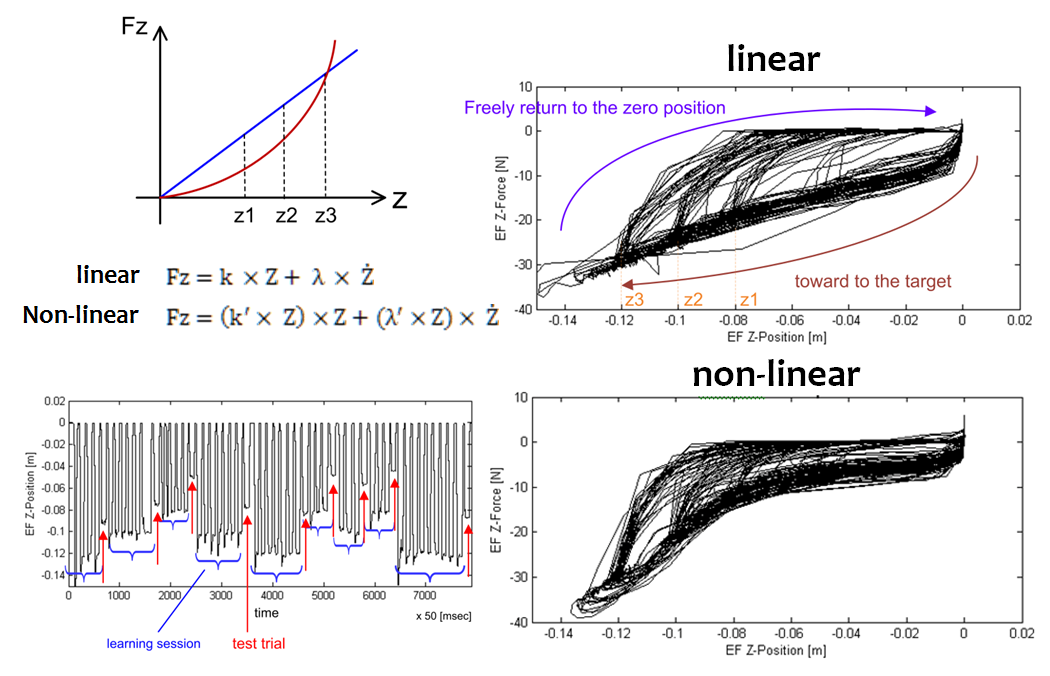
\includegraphics[scale=0.4]{Chie/figs/Figure1.png}
  \caption{The experimental design of the pilot study and the movement profile of one subject as an example. A. a cartoon of linear and non-linear force. B. time vs. z position.
C. end effector z position vs. force (linear case). D. end-effector z position vs force (non-linear case).}
  \label{expdesign}
\end{figure}


\textit{[Note: Experimental Procedure] 

The main block consisted of two parts: Learning session and Test trial. In the Learning session, the target position was coloured circle (either z1, z2, z3, randomly assigned). Participants controlled the end-effector to reach the target from the start position within a certain time window. Participant received a feedback message when they did not reach the target in appropriate timing and retried it until three consecutive movements in success before the test trial.

In the Test trial, participants moved the end-effector to the half position of the target. In this phase, no visual feedback was given to the participant in the relationship between the end-effector position and the target.

One block consists of (Learning session + Test trial) x three positions (z1, z2, z3) x 3 times = 9 trials. Participants conducted three blocks; so, 27 test trials for each task “set the half-position” and “set the half-force” in total. The experiment was completed within approximately 60 minutes on average.}

Figure 2 shows the average positions and average force in the test trials across seven participants. In the half-position task, the graph indicate that all positions overshoot than the expected position for both linear and non-linear but the non-linear case was much better than the linear case. In the half-force task, the graph illustrate that the performance was overshoot than the expected force for linear case, in contrast, the performance was undershoot than the expected force for non-linear case.
\begin{figure}
  \centering
  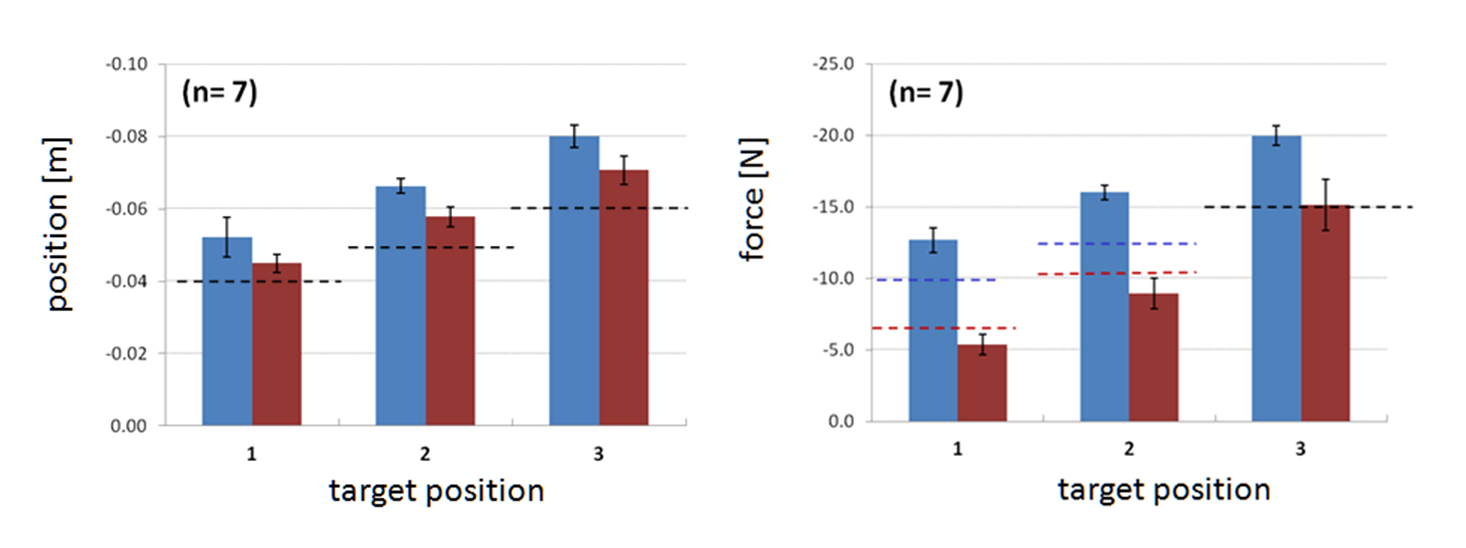
\includegraphics[scale=0.4]{Chie/figs/Figure2.png}
  \caption{The results of one version of the pilot experiment. The bar charts represents the performance. Blue bars represent the linear condition and red bars represent the non-linear condition. A. “Set the half position” task. The dotted lines indicate the ideal position. B. “Set the half force” task. The dotted lines indicate the ideal force: blue for the linear force and red for the non-linear for the linear respectively.}
  \label{pilot}
\end{figure}
We have learned human performance specifically in relation to the tasks through the pilot experiments and according to the results briefly showed above, the important factors to be considered into the experimental design are listed up, and we conducted the main experiment by adapting some changes in the protocol. 

\subsubsection{Influence of Time} 
The results indicated higher overshoots in the linear case which can be an influence of the target time window used in the previous experiments. To avoid this influence, we removed the time-window to reach the target at the training session. This will allow the participants to reach the target with slow speed and will permit exploring the force dynamics within a certain period (it’s much longer than the previous time windows).

\subsubsection{Position Accuracy vs Velocity} 
Instead of the constraint of the speed to reach the target, participants were asked to reach the target position with certain accuracy at the training session; for example, within $\pm 5$mm. If it’s over or under the range (overshoot or undershoot) at the learning session, it would be judged as an error; then participants will be asked to repeat it until the position is as accurate as possible. The participants had to reach the target position most accurately for three times (non-consecutively).

\subsubsection{Force dynamics evaluation}
To evaluate the force dynamics in terms of position accuracy and velocity, the number of reachable target is reduced to one. Three targets without a stipulated time/velocity limitations will lead to longer trials, which might be exhaustive to perform.  Instead, we proposed evaluating with four different force dynamics with one reachable target position. The testing of half-position and half-force is still considered in all the four cases.

\subsubsection{Learning model}
A learning block is introduced at the beginning of each force dynamics evaluation, to provide more trials to explore and understand the movement performed. The lack of time or accuracy limitations will make the users to learn the movement completely and further understanding the human-learning performance for different forces.

\subsection{Learning Analyses}
Human learning model for compliant contact forces and specific reachable tasks are interesting in analysing and understanding the underlying reasons behind the human performance. 

The performance and learning ability of the human in specific visual guided tasks explains the human performance in dynamically compliant contacts \cite{ernst2002}. This learning model helps in understanding the human impedance behaviour which can further help in improving the robot performance. This also helps in identifying the human-robot interaction model to be developed and used in creating a human friendly robot. 

Humans perceive the applied force based on the input from the contact model and the compliance of the system \cite{pongrac2006}. To understand the influence of the human behaviour in different force model applications it is important to understand the impact of such forces and the learning model of the human interaction. The human force interaction model is also a subjective model depending on  each human subject’s ability and involvement in the interaction. Indeed, the interaction can be limited by defining a target position model to be reached and the velocity to be maintained while maintaining the target position.

This learning analysis helps in understanding the human-force perception or how humans perceive the different force dynamics, provided there is a position limitation. Further, it explains if they can differentiate (cognitively) the force models and their applied effort. This led us to further analyse how individual perception vary or if they can relate this force models to any activity for daily living scenario. Moreover, it is interesting to compare the human perception both verbally and cognitively to understand how the human perception model works. Including a simple questionnaire is another way to understand the human haptic force perception model, especially in relation to the forces applied in any daily activity \cite{van2014}. The questionnaire involves multiple real life scenarios which can explain the linear and non-linear forces.

\subsubsection*{Dynamic learning evaluation}
The dynamic learning metric evaluation is performed using the target position maintained with a constant velocity at the end of the goal position.

Metrics for dynamic learning analysis:
%
\begin{equation}
  M=Z-Z_d +K* (\dot{Z}-\dot{Z_d})
\end{equation}
%
Z is the target position reached at the end of each trial and $\dot{Z} $ is the velocity maintained at the target position; $Z_d$  and $\dot{Z_d }$  are the desired goal position and velocity respectively. K is a constant value defined as function of the output sampling rate. The sampling rate function with the velocity parameter will explain the change in the target position adding some more windows to be more accurate.  The goal of this analysis is to observe the number of trials needed for each user to reach the target position as accurate as possible, provided the velocity is maintained at zero, at the end position.
	
The objective of this learning model is to understand the human perception and precision in reaching a specific target position. There was no time limitation to reach the target position, providing the users have enough chances/time to understand the different forces. 

\subsection{Methods}

\subsubsection{Apparatus and stimuli}
Similar to the initial pilot experiment, the current study employed a haptic device, Haptic Master (Moog, Inc.), which consisted of a large robotic rod with an end-effector. The device is controlled by a set of computer programmes to render robotic manipulandum for force feedback. We measured the end-effector movements controlled by human subjects and analysed the dynamic properties of the movements against the compliant force and the performance. The forces and the movements were constrained in vertical (Z) direction to the ground only.

We used the ready-made spring model in the Haptic API, where the compliant force formula was assigned to the device. The compliant force was rendered by sending parameters (i.e. spring stiffness and damping factor) in real-time depending on the end-effector position and the velocity (Figure 3).

%
\begin{figure}
  \centering
  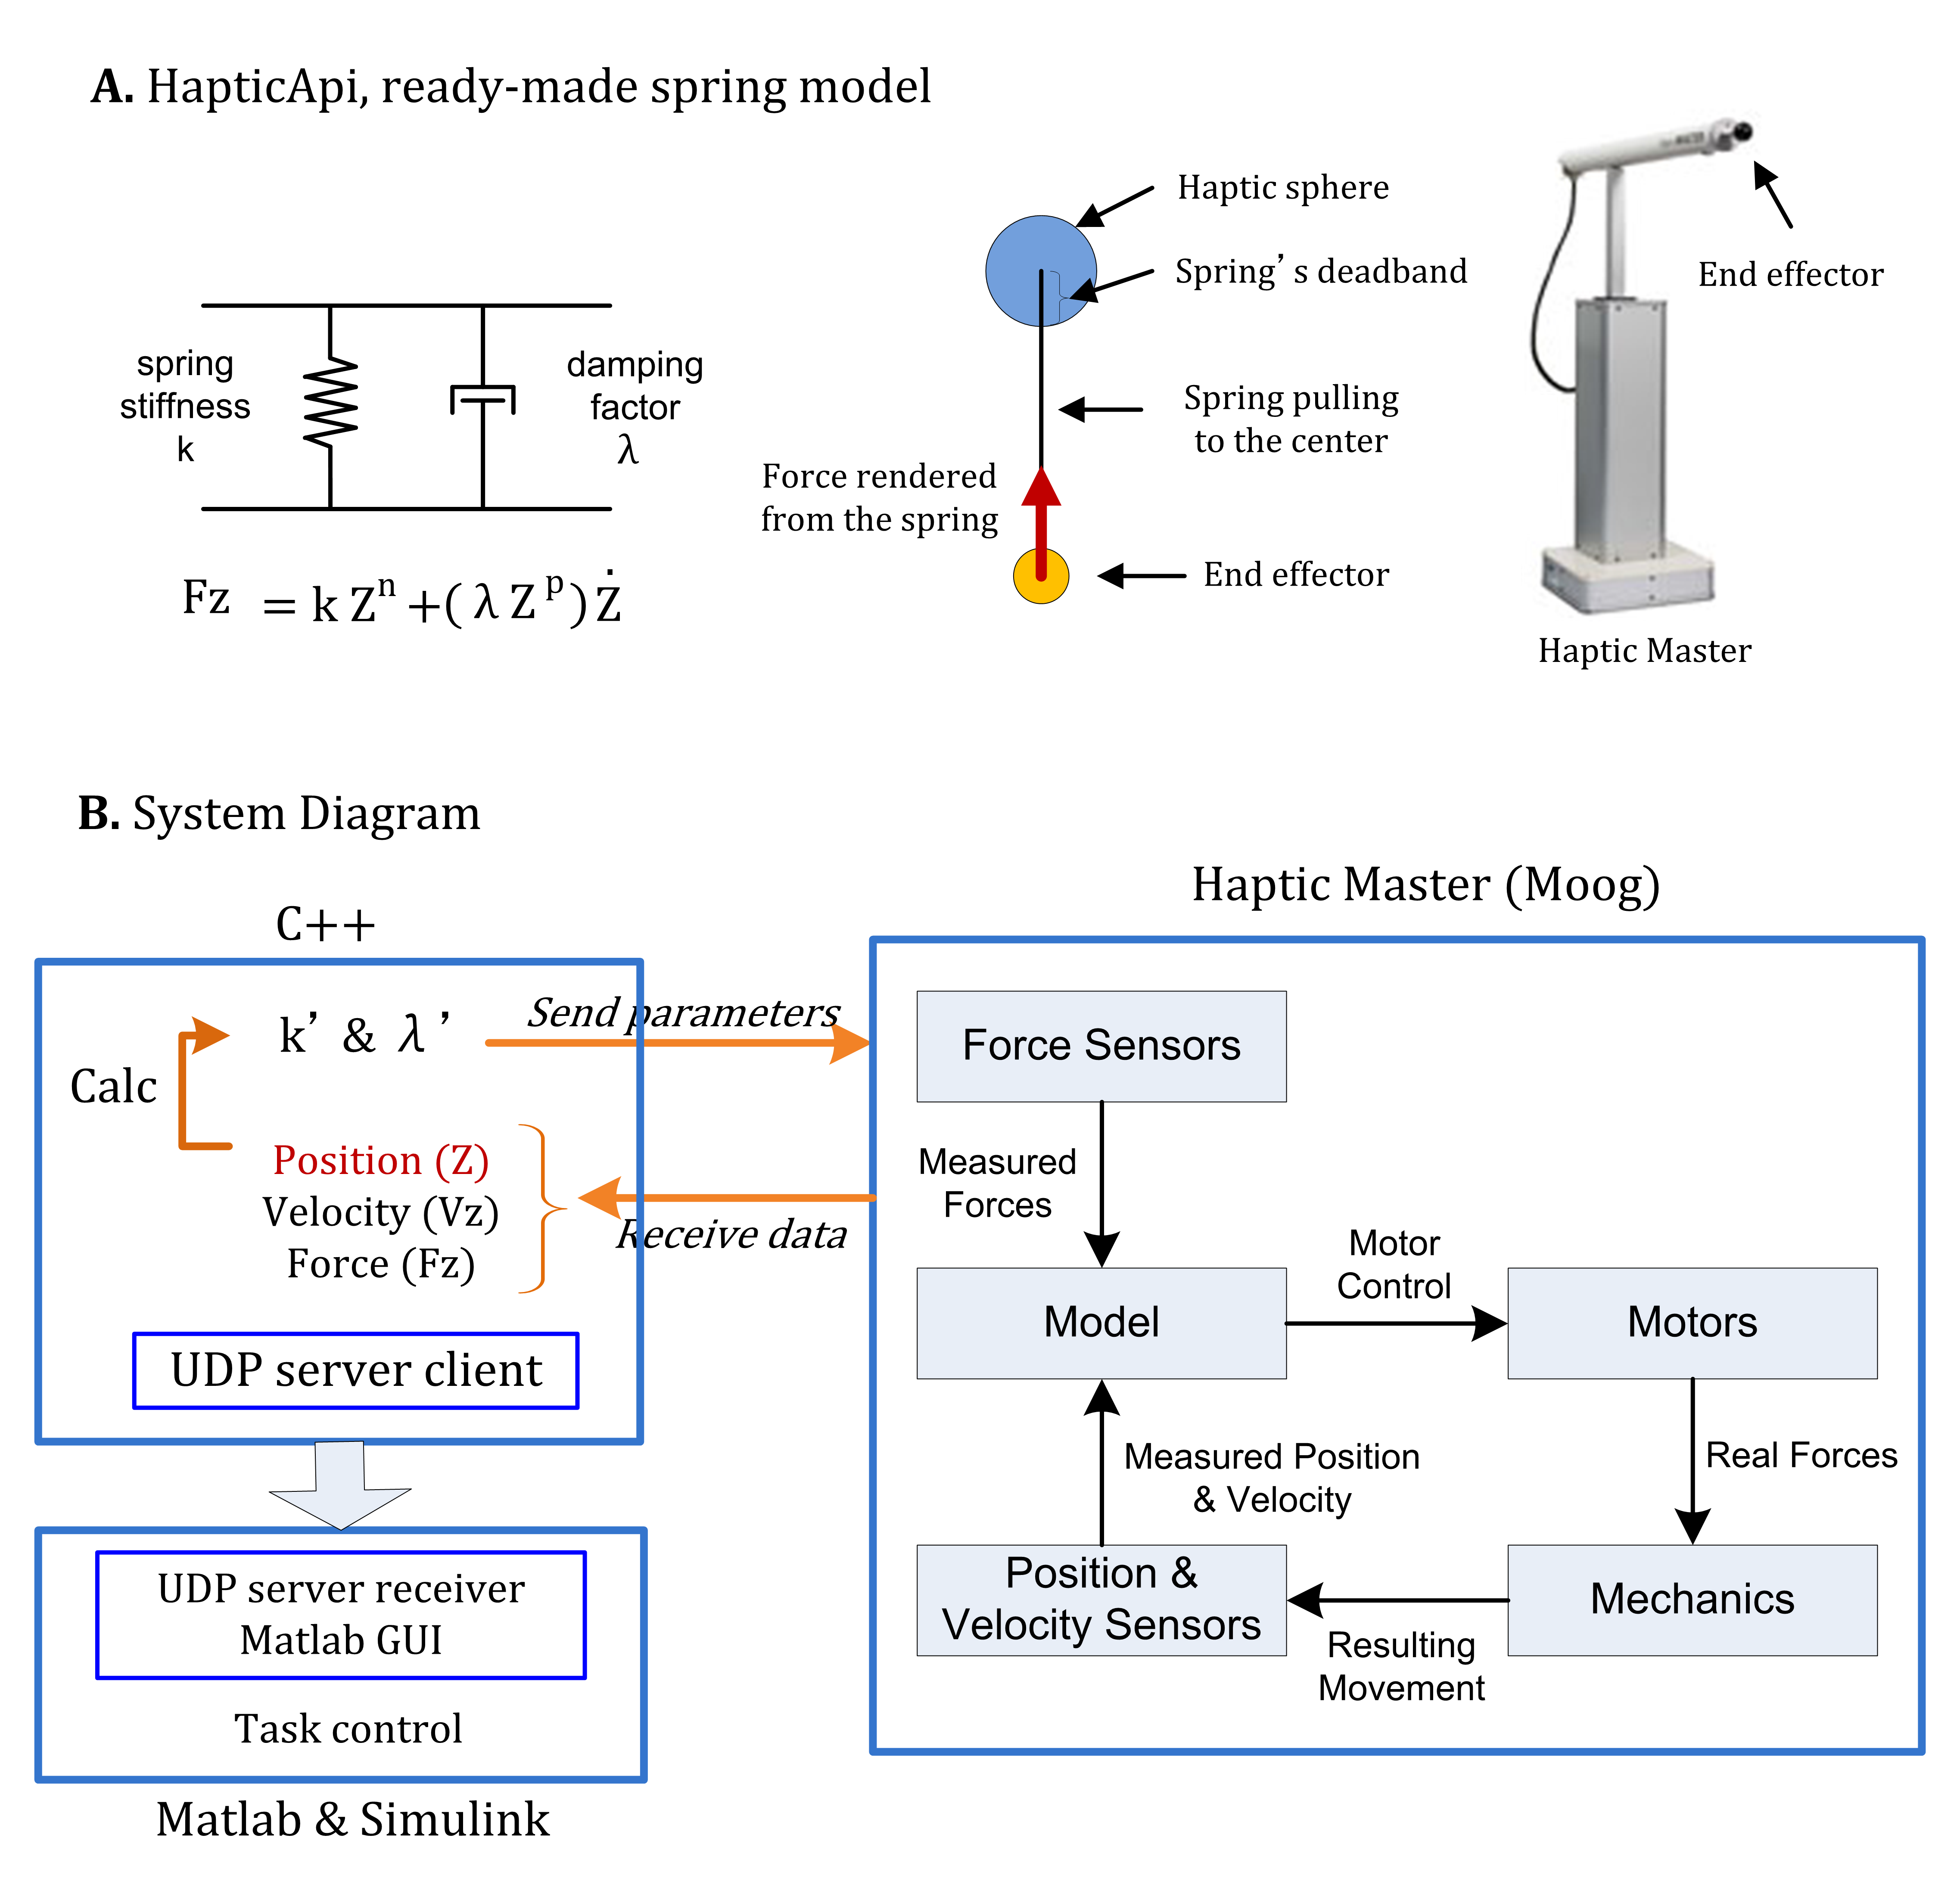
\includegraphics[scale=0.5]{Chie/figs/Figure3.png}
  \caption{A. The ready-made spring model in the Haptic API. B. A block diagram of the compliant force control. The force is rendering based on the end-effector position and the velocity with parameters (spring stiffness and damping factors) in the real time.}
  \label{modelling}
\end{figure}

\subsubsection{Experimental Design}

\paragraph{Different force dynamics}
In general, spring-damper force ($\BF$) is formulated by the position and the
velocity with parameters: spring stiffness ($k$) and spring damping factor
($\lambda$).  Here, it is simplified for one direction ($\BZ$).
%
\begin{equation}
  \BF = k \BZ^n + (\lambda \BZ^p) \dot{\BZ} \, .
\end{equation}
%
We generated four different compliant forces (two linear and two non-linear cases) by changing the stiffness k values (see Figure 4 and Table 1). The k value is maintained constant in linear case and position dependent in case of non-linear forces. In Figure 4, the linear cases are [1] and [4], and the non-linear cases are [2] quadratic and [3] concave, respectively.
\begin{figure}
  \centering
  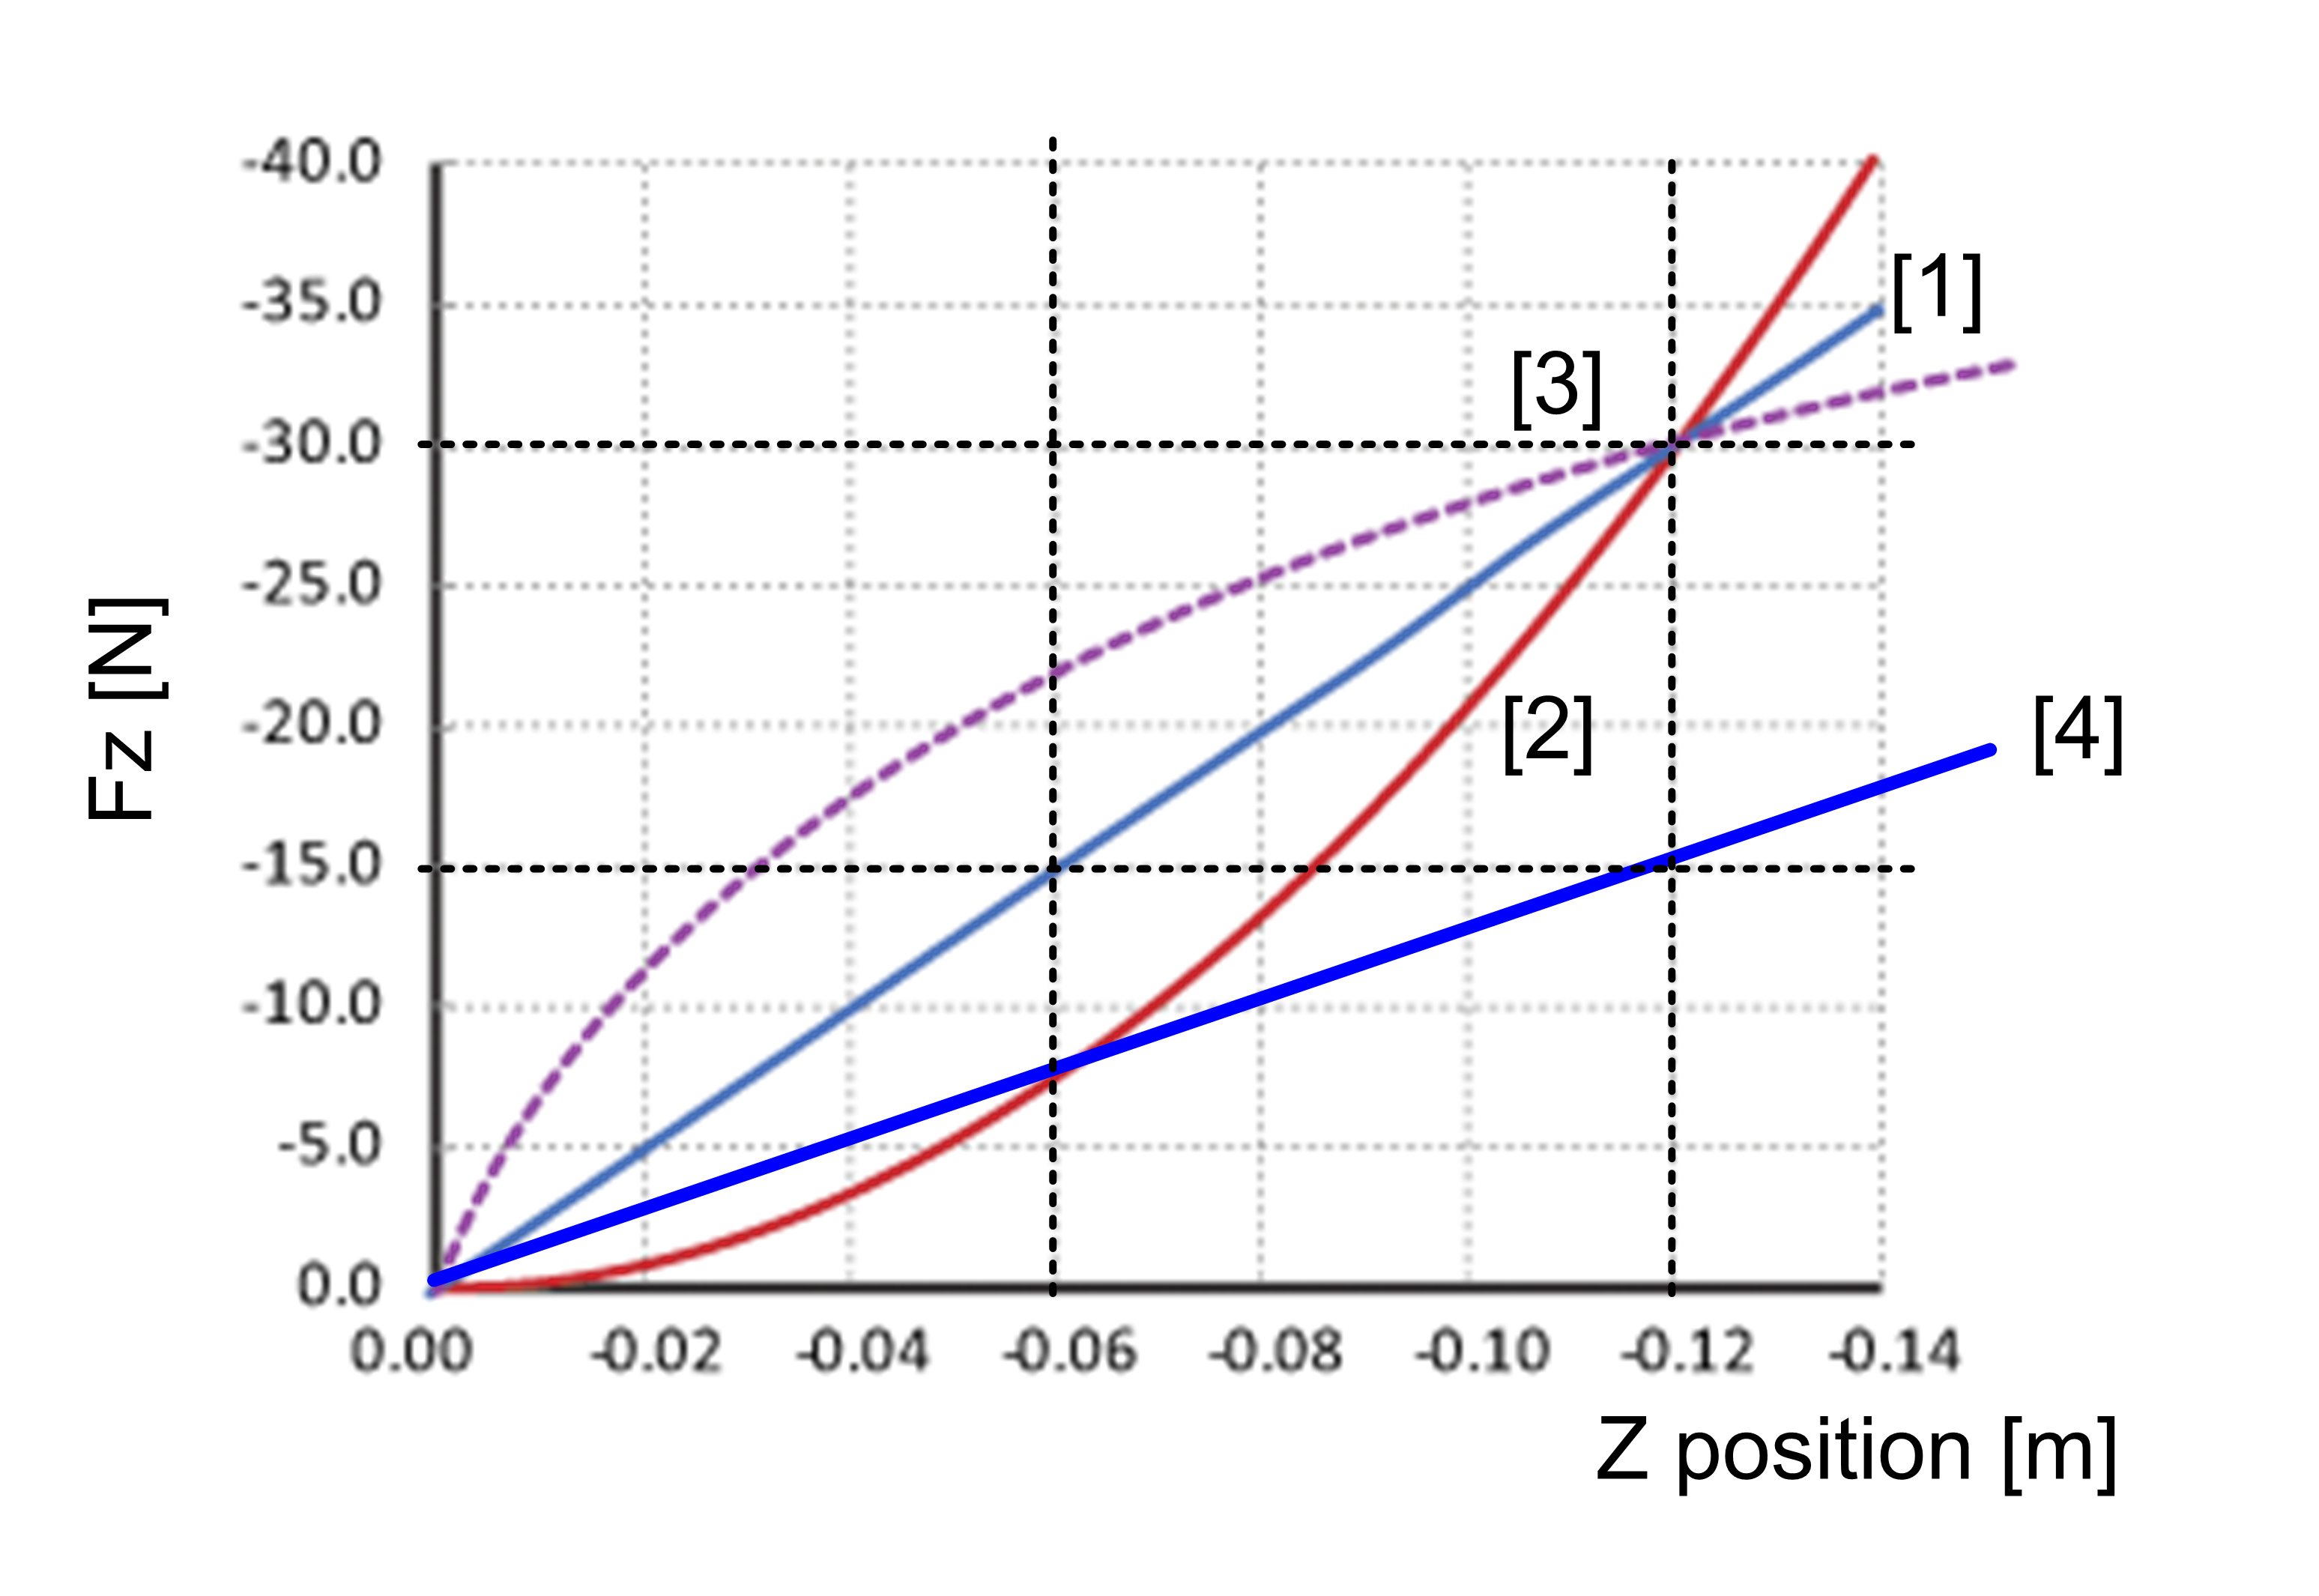
\includegraphics[scale=0.5]{Chie/figs/Figure4.png}
  \caption{Four different force dynamics are applied. [1] Linear, [2] Non-linear (quadratic), [3] Non-linear (concave), and [4] Half-linear. The [1],[2],[3] are the same force at the end position (e.g., z=-0.12), and [2] and [4] are the same force at the half position  (e.g., z=-0.06).}
  \label{forcedyn}
\end{figure}

\begin{figure}
  \centering
  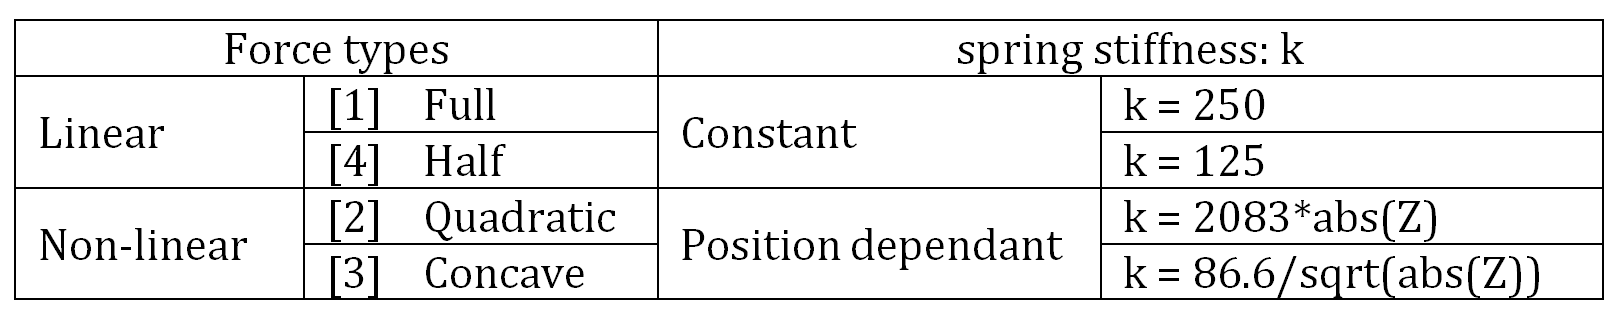
\includegraphics[scale=0.4]{Chie/figs/Table1.png}
  \caption{Table 1. The four different forces are rendered by changing the spring stiffness. See the parameters in the table.}
  \label{Table1}
\end{figure}

\paragraph{Questionnaires}
The questionnaire (Q1 and Q2) we introduced to this experiment can be seen in Table 2. It is interesting to compare the human perception both verbally and cognitively to understand how the human perception model works. A simple questionnaire to rate the effort to deal with the applied force (Q1) is a way to understand the human haptic force perception model \cite{tan1994}, compared with the individual physical performances. Moreover, it is beneficial to examine the force perception in relation to the forces applied any daily activities (Q2). The questionnaire involves multiple real life scenarios which can be explained by the linear and non-linear forces. Individual subjective responses to this questionnaire would also help to understand human physical performance and also bridge the relationship between human motor control against the force and the subjective force perception.
\begin{center}
\caption{Questions and responses. This questionnaire was introduced to examine human haptic force perception after a certain exposure to the repetitive movements against a specific compliant force. All questions were repeated at the end of each session.}
\begin{tabular}{ c ¦ c  }
Questions & Responses \\
Q1.Rate the applied force in terms of effort. & 1. Extremely Low
& 2.	 Low
&3.	 Moderate
&4.	 High
&5.	 Very High \\
\hline
Q2.	How do you relate this force with a common day-to-day activity? & a.	 Pushing a cushion
& b.	 Pushing a revolving door
& c.	 Pushing a box on a plane surface
& d.	 Pushing a hinged door
&  e.	 Pushing a box on an inclined surface\\
\hline
\end{tabular}
\end{center}

\subsubsection{Experimental Protocol/Procedure}

\paragraph{Protocol}
Based on the pilot experiments conducted and the in-depth analysis of the result, a detailed experimental protocol was designed as illustrated in Figure 5. Initially, a Practice Session was introduced using only the half-linear force to learn the complete task. Following the practice session, Three different force sessions (linear, quadratic, and concave) were “pseudo-randomly” assigned. The random order aimed to minimise the order effects on the performance.
\begin{figure}
  \centering
  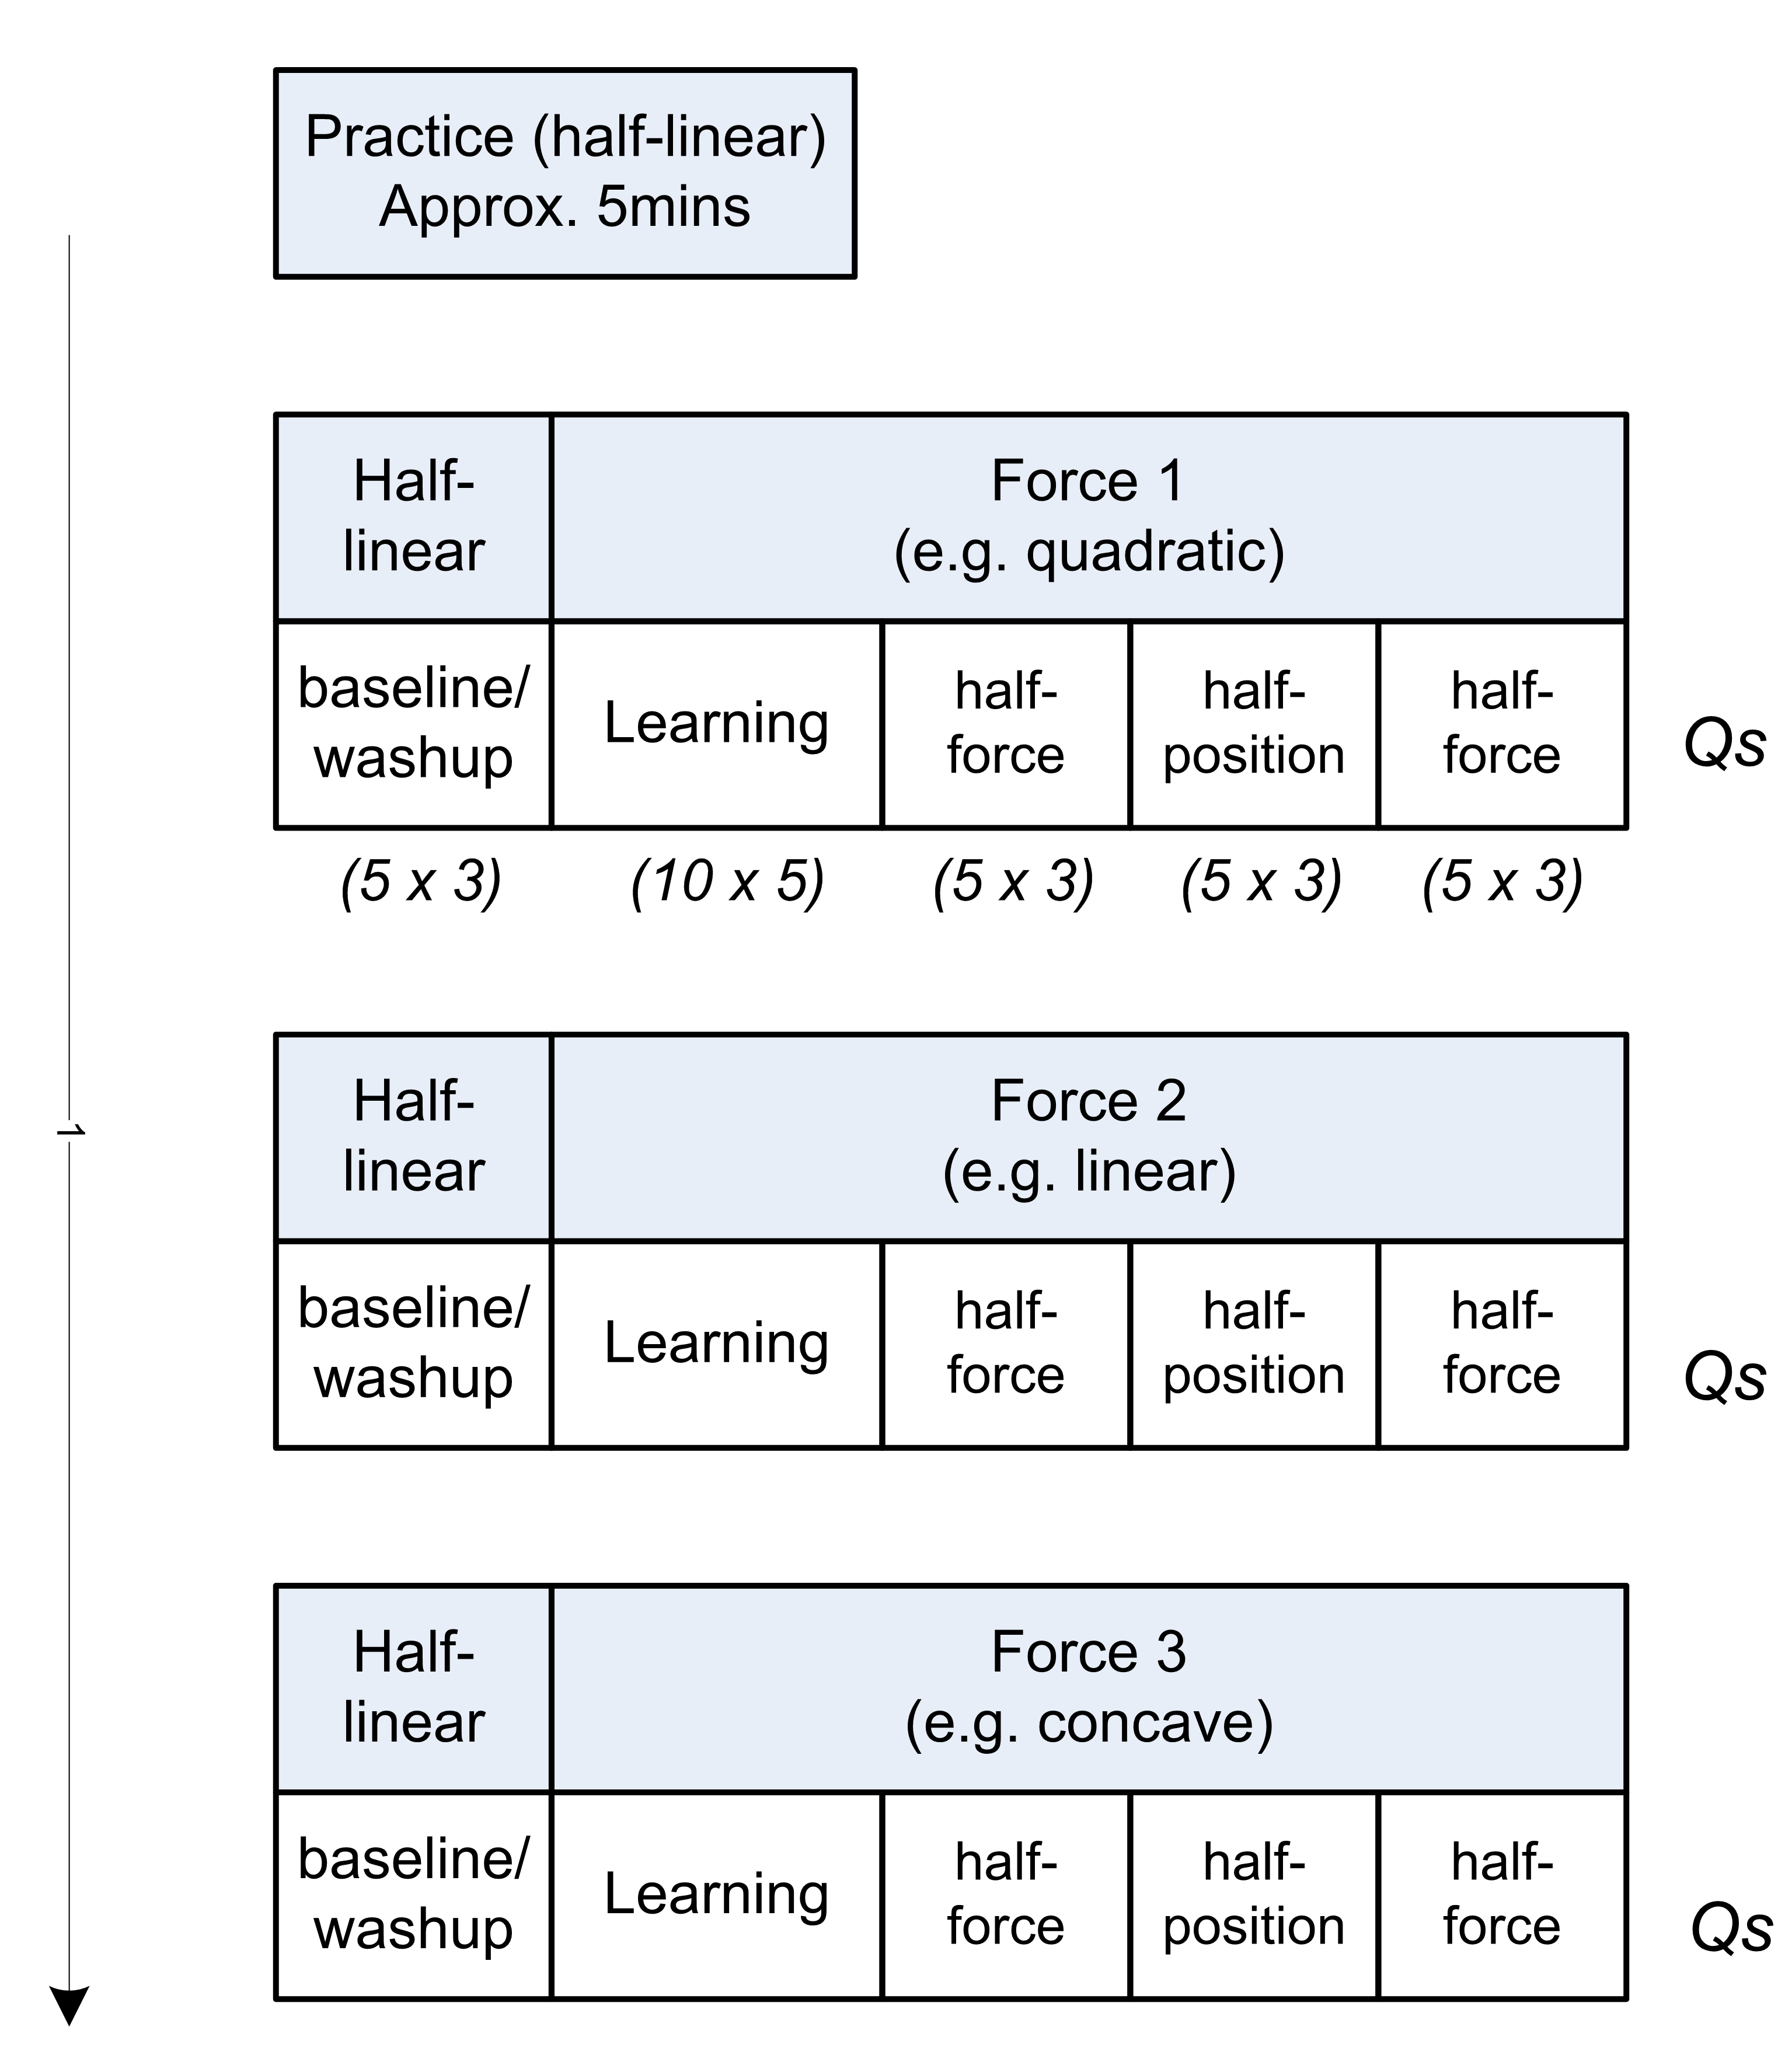
\includegraphics[scale=0.5]{Chie/figs/Figure5.png}
  \caption{Experimental protocol. Approx. 5 mins practice session followed by three sessions with different (one linear and two non-linear) forces. Each session started with baseline/wash-up and learning blocks and then three test blocks. More details can be seen at the main text.}
  \label{protocol}
\end{figure}
Each session consisted of a series of five blocks (baseline/wash-up, learning, half-force, half-position, and then half-force). In all the blocks, there were a certain number of test trials. The test trials probed whether participants could appropriately produce either half-force or half-position of that they previously learned through their repetitive movements to reach the target.

-	The “half-linear” force block was set at the beginning of each force session as a baseline/wash-up. “The test trial asked a participant to set the force of the target previously learned” after five repetitive movements to reach the target position.
-	In the “learning” block, there were ten test trials: “Set the force of the target previously learned” after five repetitive movements to reach the target position.
-	In the “half-position” block, there were five test trials: “Set the half-position of the target previously learned” after three repetitive movements to reach the target position.
-	In the “half-force” block, there were five test trials: “Set the half-force of the target previously learned” after three repetitive movements to reach the target position.
-	The half-force block was conducted twice; so the total was 10 test trials.

After the completion of each session, a participant took a break and was asked to answer a few questions aiming to assess subjective perception to the force he/she experienced.

\paragraph{Procedure}
At the beginning of the experiment, all participants received the instruction from the experimenters. After understanding the task well, a participant stood in front of the haptic device and grasped the end-effector.

The “Home” position, where was the centre of the end effector is z = 0 at the workspace, was 110 cm from the ground. The spring position was set at z = 0. In this study, the rod movements were restricted in the vertical direction only. The target positions were set at z = 120 mm.

The visual information about the task was provided at the computer display to human subjects.
The computer screen was located in front of human subjects; where the centre of the screen was align to the centre of the robotic rod. The screen was approximately 1.60m away from the participants’ standpoint. Height from ground- approx.162cm, screen display size 531.36mm (Ht) x 298.89mm (W). The screen displayed the target position and the end-effector position in real-time, excluding the test trials (Figure 6). 
%
\begin{figure}
  \centering
  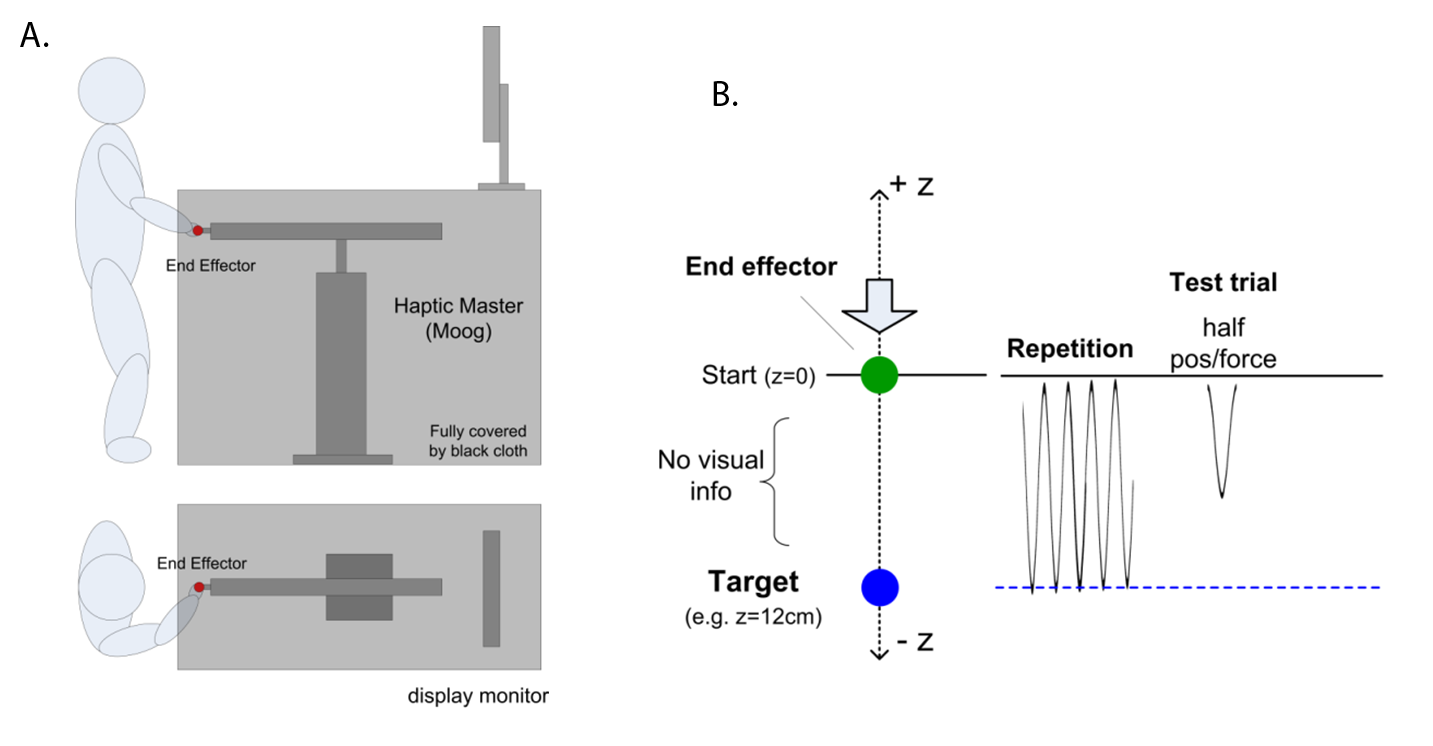
\includegraphics[scale=0.5]{Chie/figs/Figure6.png}
  \caption{A. A cartoon of an experimental setting. B. The explanation of the experiment. The end-effector and the target positions were visually indicated on the computer screen during the repetitive period, but there were no visual info at the test trial. .}
  \label{settingHM}
\end{figure}

Based on the experimental protocol as described above, all participants begin with the practice session followed by the main sessions. They were required to make repetitive movements against the compliant force generated by the haptic device to learn kinetic principle. Participants pushed the end-effector to reach the target position, and then released the end-effector to allow it to freely return to the initial position (z = 0). The end-effector movements were monitored by the computer systems and the visual information was provided on the screen, excluding between the start position and the target position (See Figure 6 B.) The target zone was visually defined by a coloured circle. The colour was controlled by the Matlab/Simulink computer programme and changed depending on the condition, aiming to inform the condition to participants. 

In the repetitive period, participants were asked to reach the target position$ (z = -0.12 m)$ within a certain time window $(0.6\pm 0.2s)$ as accurate as possible. The timer started when the end-effector moved from the initial position and stopped when the end-effecter position crossed the target position.  Participants received the feedback message for the each movement on the display:  “too fast” when $< 0.4 s$, “good timing” $0.4s \leq t \leq 0.8 s$, and “too slow” when $t > 0.8 s$. They were also requested to set the end-effector within the target zone as accurate as possible and to keep it staying there for approx. 1 sec, ideally maintaining it with zero velocity.

In the test trial, in the “practice” and “learning” blocks, participants were asked to set the end-effector at the same feeling of the force at the target previously learned after the repetitive movements. In the “half-force” block and the “half-position” block, the test trials asked participant to set the end-effector at the same feeling of the half-force or the half-position, respectively. They were requested to keep the end-effector there with no visual feedback and to maintain it with zero velocity for approx. 2sec.

In order to help the participants concentrate in the force analysis and the compliance, an alpha noise was introduced to the users. The participants had headphones on which also helped in removing the external or any environmental disturbances and to concentrate on the experiments.

\subsection{Results and Discussion}
\subsubsection{Participants}
Eighteen subjects (age range: 18 ~ 41,) took part in the experiment (12 female, 18-41 years old, mean age: $20.4 +/- 5.2 (SD)$, mean height: $169.1 cm +/- 8.8 (SD)$, 14 right-handed). All the participants had normal or corrected to normal vision, and no known motor deficits and/or any limb injuries by self-reported. The study was approved by the Research Ethics Committee, University of Birmingham, and all procedures were in accordance with the Declaration of Helsinki. Participants were recruited via the University Research Participant Scheme – SONA System . Subjects gave informed consent to participate, but were naïve to the purpose of the experiment. They also have no prior knowledge about the system or the force models chosen.

\subsubsection{Responses to the three different force dynamics in the test trials}
The sensorimotor physical properties (e.g. distance, velocity, and force) were collected through sensors, mounted at the end effector, while the human subjects were controlling their movement under different force dynamics were applied. The dynamic properties of the point-to-point movements were measured: the end-effector’s position (z), the velocity $\dot{z}$, and the force (Fz) across the time. These were recorded by the 20Hz sampling rate. We read-out the data (position and force) at the test trials in the “half-position” task and “half-force” task and analysed the differences between the three different force conditions. Figure 7 shows one of the participants performance as an example.
%
\begin{figure}
  \centering
  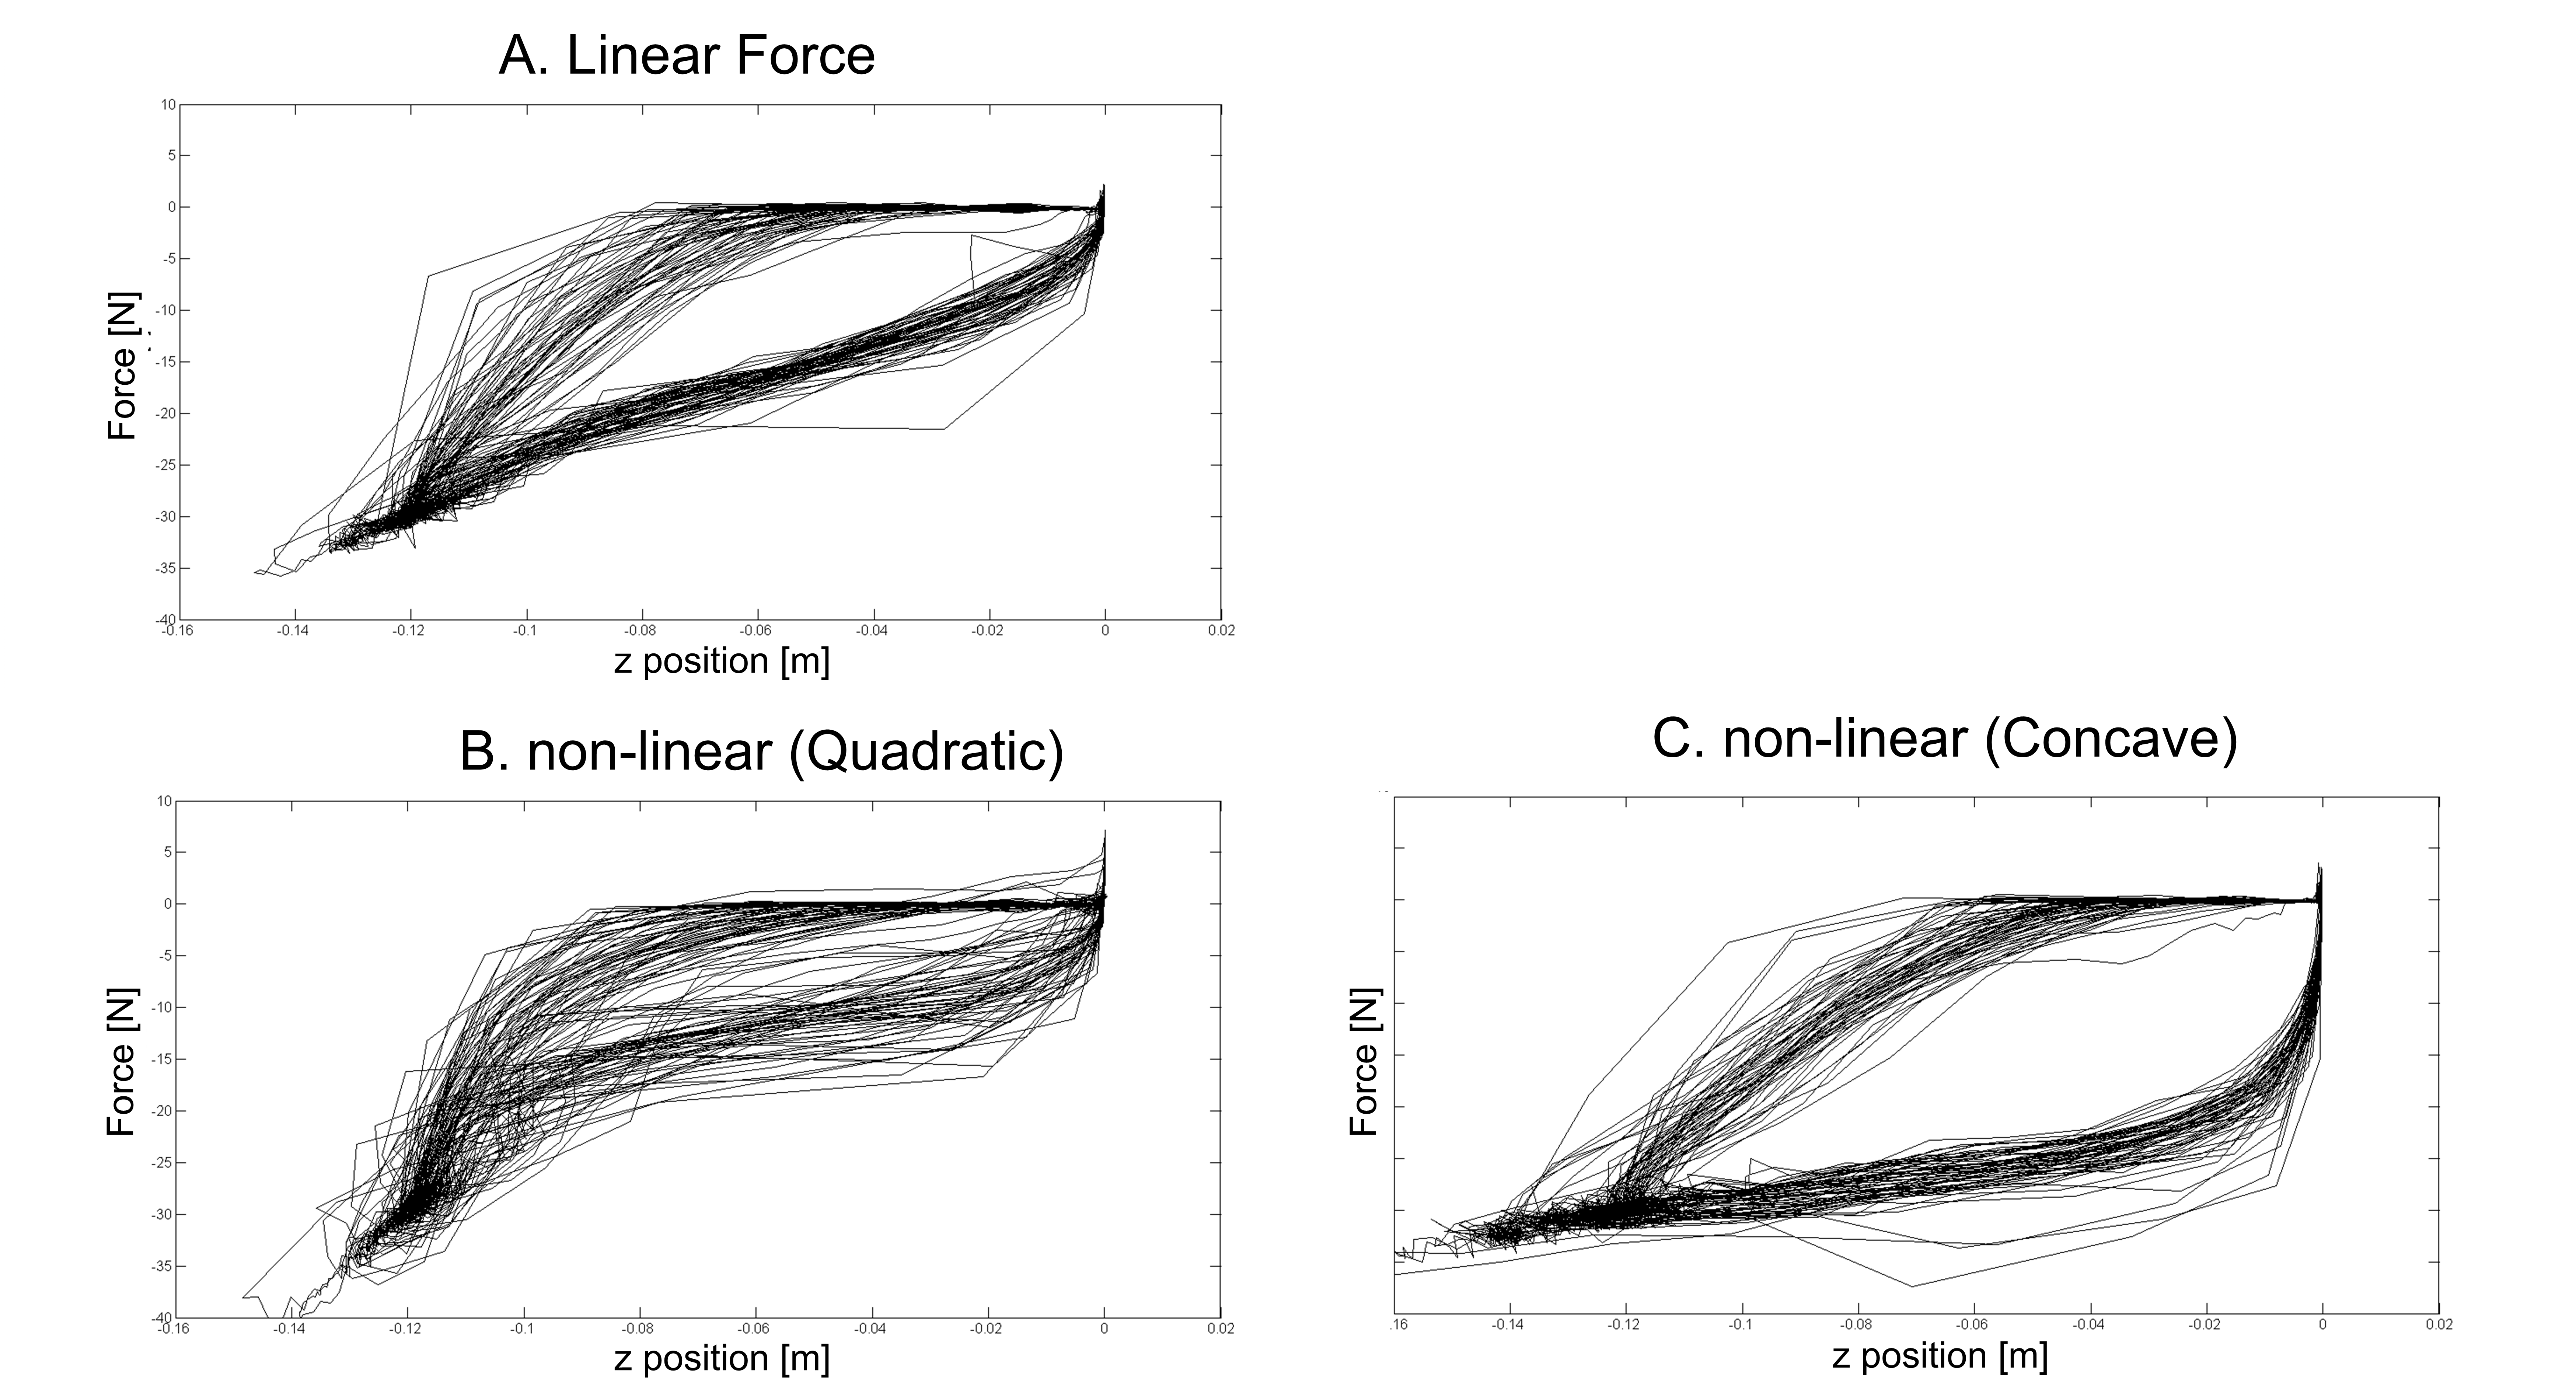
\includegraphics[scale=0.5]{Chie/figs/Figure7.png}
  \caption{An example of one participant’s movement profile. The three graphs represent the properties of the movements (position vs force) under three different conditions. A. linear, B. quadratic, and C. concave.}
  \label{modelling}
\end{figure}
\paragraph{“Set the half position” performance}
Figure 8 shows the averaged performance across 5 test trials in the “half-position” task. In this task, participants kept the end-effector at the similar position which they felt as the half-position in the previous repetitive movements. Therefore, we evaluate how they accurately move the end-effector compared with the “target” half position.
%
\begin{figure}
  \centering
  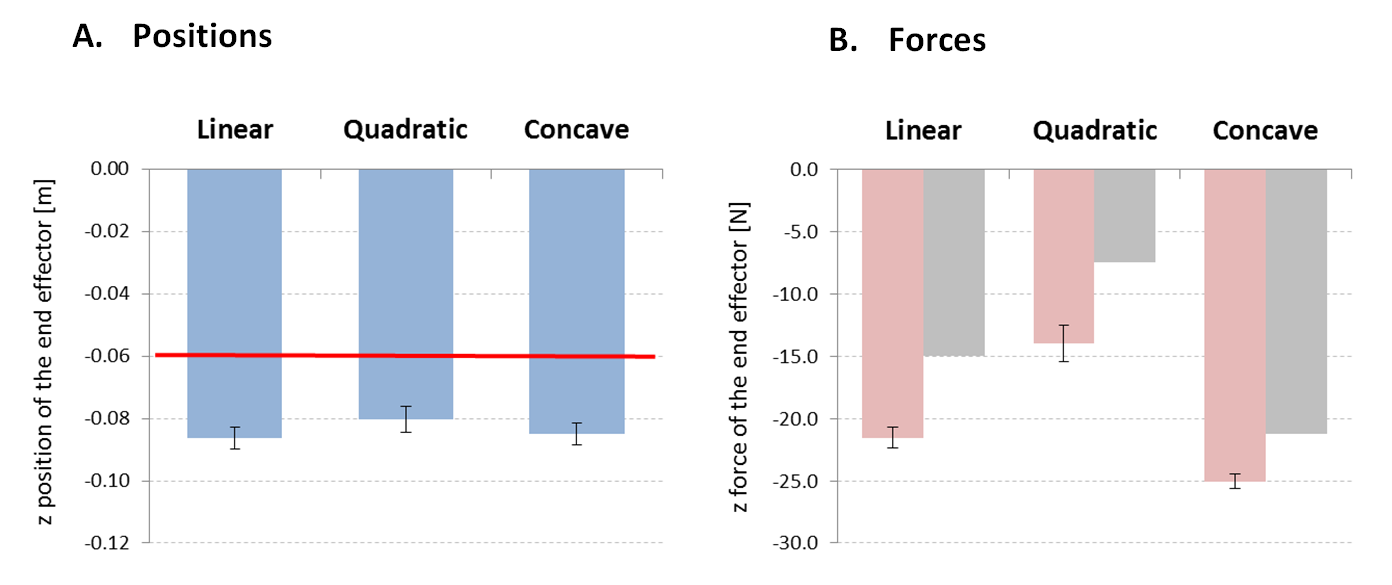
\includegraphics[scale=0.5]{Chie/figs/Figure8.png}
  \caption{The end-effector position and force at the test trial, averaged across 18 participants. 
A. the positions for three different force conditions, compared with the red line representing the ideal position z = -0.06 [m]. B. the force for three different conditions, compared with the grey bars representing the “target” force (see Figure 4).}
  \label{testrial}
\end{figure}
According to the Figure 8A, an overshoot  from the target position $(z = -0.06 m)$ is observed for all the three conditions. This overshoot can be considered as the effect of the deprivation of visual-feedback in the test trials because the same performance was observed at the wash-up/baseline and learning blocks.

There were no significant position differences between three force conditions. A statistical analysis supports this. Mauchly’s test of Sphericity indicated that the assumption of sphericity had been violated, $χ^2 (2) = 9.429, p = .009 < .05, $ therefore degrees of freedom were corrected using Greenhouse-Geisser estimates of sphericity $(\epsilon = .69)$. The results show that there were no significant differences on position perceptions under different force dynamics was applied, $F(1.384, 23.524) = 1.501, p = .240$.

\paragraph{“Set the half force” performance}
Figure 9 shows the averaged performance across 10 test trials in the “half-force” task. In this task, participants kept the end-effector at the similar force as much as possible which they felt as the half-force in the previous repetitive movements. Therefore, we evaluate how they accurately move the end-effector compared with the “target” half force. 
%
\begin{figure}
  \centering
  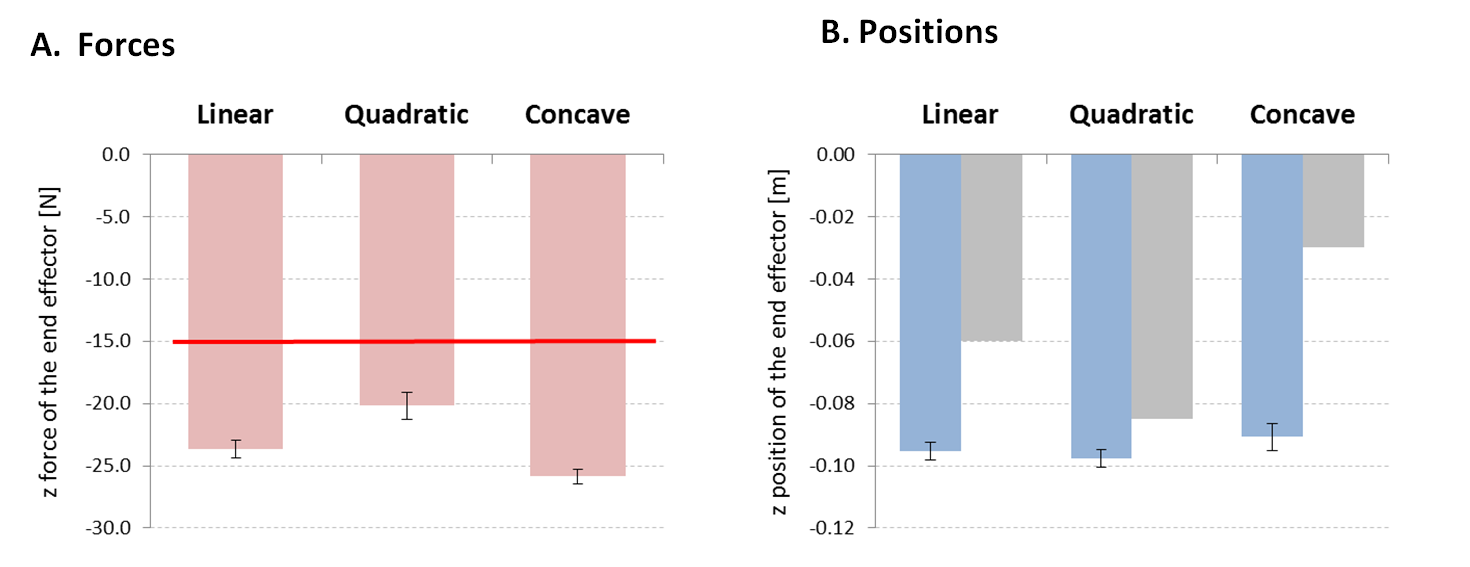
\includegraphics[scale=0.5]{Chie/figs/Figure9.png}
  \caption{The end-effector force and positions at the test trial, averaged across 18 participants. 
A. the forces for three different force conditions, compared with the red line representing the targeted force Fz = -15 [N].  B. the positions for three different conditions, compared with the grey bars representing the “targeted” force (see Figure 4).}
  \label{half-force}
\end{figure}
According to the Figure 9A, overshoot in forces  from the target force (Fz = -15.0 N) was also observed for  all the conditions. This overshoot also can be considered as the effect of the deprivation of visual-feedback with the same reasons as discussed above at the position task.

Figure 9A shows that there were significant differences between the three force conditions. Further statistical analyses were made. Mauchly’s test of Sphericity indicated that the assumption of sphericity had been violated, $χ^2 (2) = 8.221, p = .016 < .05$, therefore degrees of freedom were corrected using Greenhouse-Geisser estimates of sphericity $(\epsilon = .71)$. The results show that there were significant performance differences in the half-force task under different force dynamics, $F(1.427, 24.255) = 27.165, p = .000$.

\paragraph{Work of a force analyses}
The read-out positions and forces, as analysed above, might not well represent the influence of the force dynamics on the performance because of the pinpoint values. Here, we consider the influence by the exposure of the force dynamics for the movements and tried to conduct further temporal analyses.
%
\begin{figure}
  \centering
  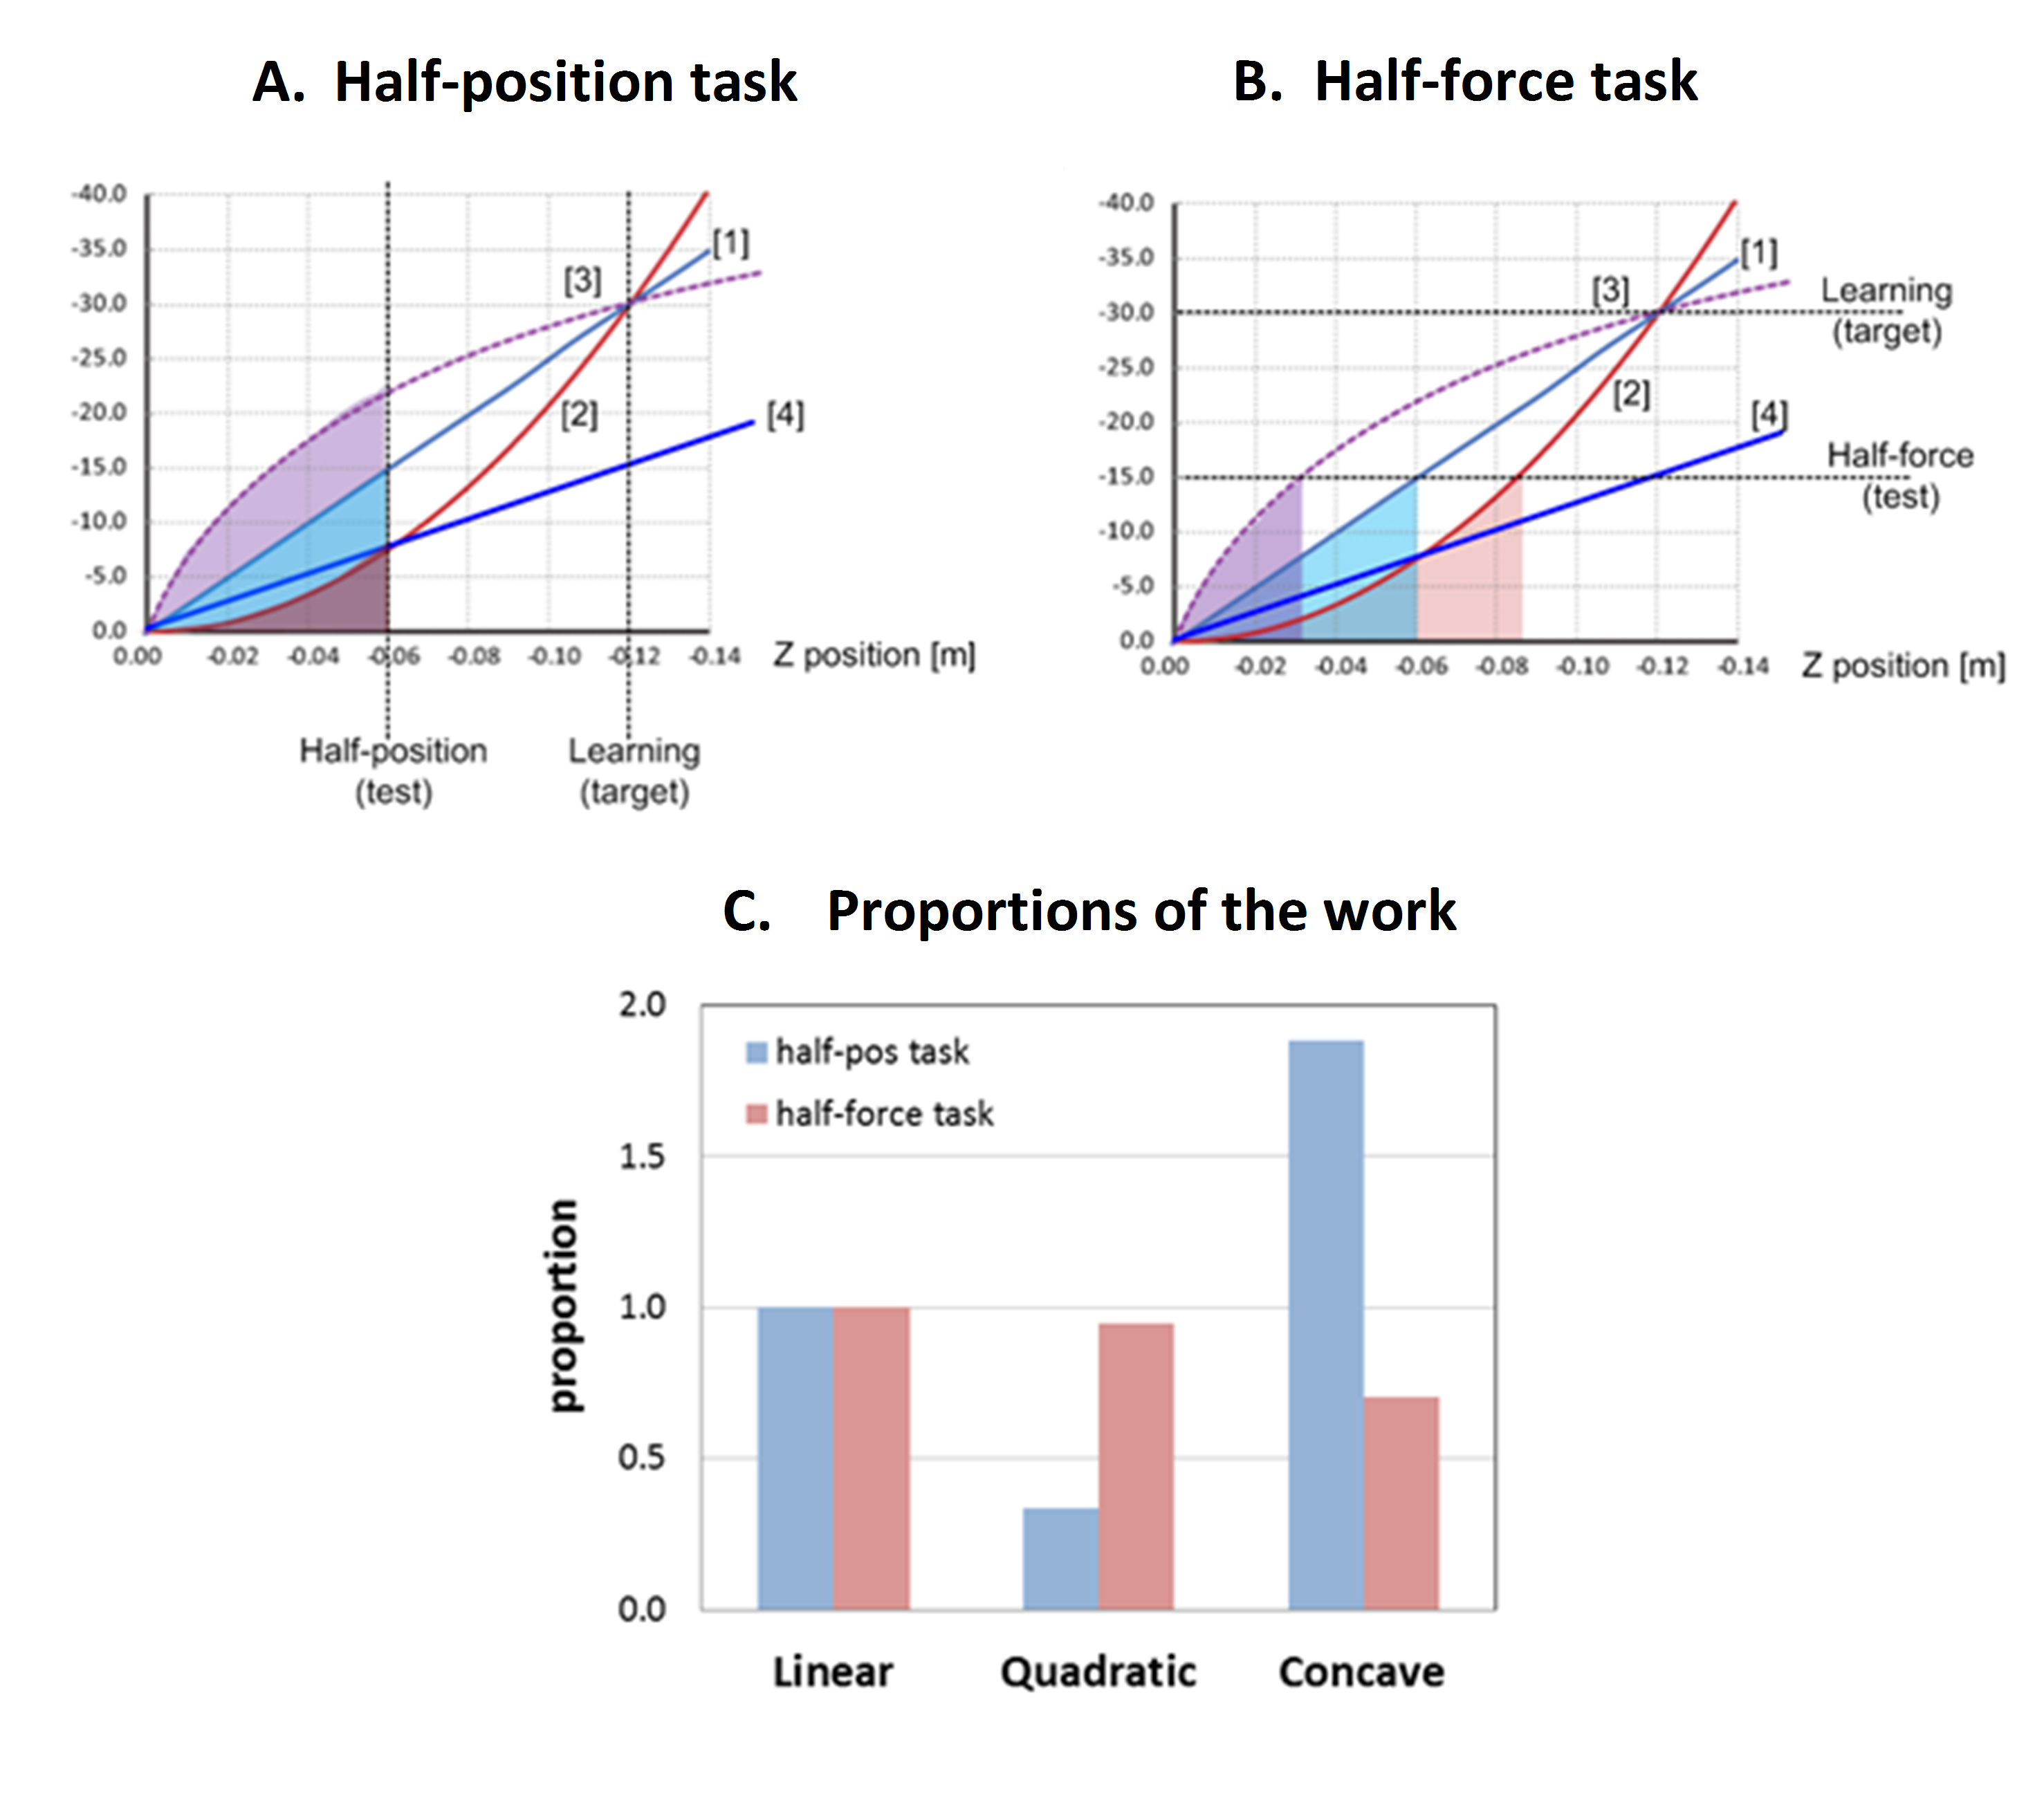
\includegraphics[scale=0.5]{Chie/figs/Figure10.png}
  \caption{Illustrations to explain the Work differences for the half-position task (A) and the half-force task (B). Coloured areas represent the Work depending on the force dynamics. C. the bar charts of the proportion of the work when linear work is 1.0. }
  \label{work}
\end{figure}
The definition of “Work” is the result of object movements against force. Work of a force can be calculated by the line integral of its scalar tangential component along the path (from z1 to z2).

%
\begin{equation}
  \BW = \int_{z1}^{z2} f(z) dz
\end{equation}
%

Based on the Figure 4, the Work should be different between three different forces.
Figure 10 shows that there are significant differences on the Work when conducting half-position task than half-force task.

Based on the measurements (position, velocity, and force for each conditions), we calculated the temporal aspects of the tasks with the different force dynamics.
%
\begin{equation}
  \BW = \int_{t1}^{t2} fz Vz dt
\end{equation}
%

In Figure 11, the similar pattern between three force dynamics can be seen for the all the three sessions: learning, half-position, and half-force tasks. Such energy pattern might affect the half-force task performance and some participants might set the end-effector at half-energy they felt rather than the half-force itself. This pattern can be confirmed by the significant differences between the three forces in Figure 8. Humans might be not good at the point perception of the force, but the brain might be better understanding of the total cost and employ it to estimate/predict the “half” force ruled by the energy. To evaluate these possibilities, we need further data analyse and may be required to conduct additional/supplemental experiments.
%
\begin{figure}
  \centering
  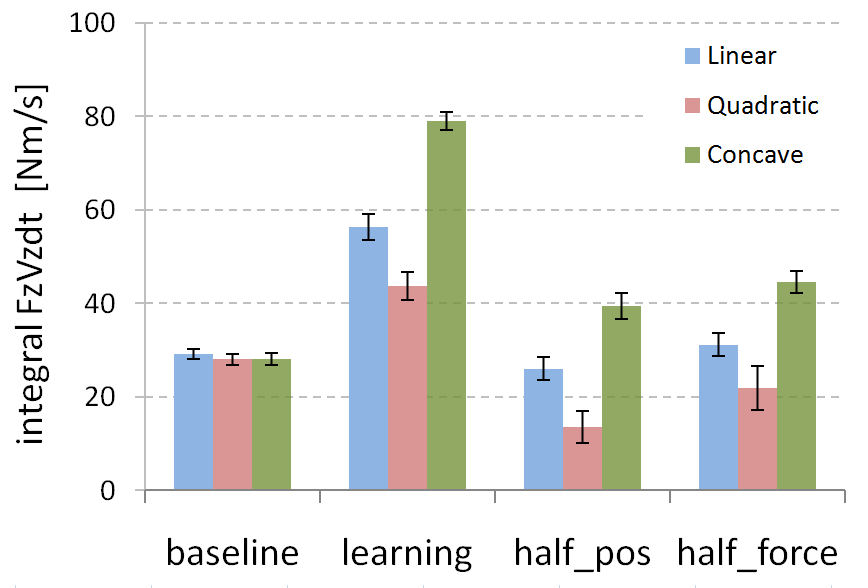
\includegraphics[scale=0.5]{Chie/figs/Figure11.png}
  \caption{The calculations from the measurement values (force and velocity) from start to the end points at the test trials, averaged across 18 participants.  Note: in the baseline block, only the half-liner force was applied.}
  \label{forcevel}
\end{figure}
\subsubsection{Dynamic learning evaluation}
The dynamic learning performance of human reachability tasks was evaluated and the results of 18 participants are presented and discussed in this section. The sequences of the three forces which are applied are different for each user (the order was pseudo-randomly assigned to the subjects and well counter balanced between them.) This consideration could help in understanding the role of each force models and the learnability for three different forces and also to see whether they affect any part of the learning model.

In the learning session, the user repeated the target reaching movement for n=50 trials. The averaged learning performance of the 18 participants depicted the behaviour pattern observed against a target position reached and maintaining them at a constant 0 velocity at the end the movement. 
In the analyses, we set the parameters to the equation (2) as below.
$Z_d=0.12  m;\dot{Z_d}=0.0  m/s;K=0.05 s ;$
K is a constant value defined as function of the output sampling rate.

The K value is defined as function of the output sampling rate (in Simulink). The goal of this analysis is to observe the number of trials needed for each user to reach the target position and also maintaining a zero velocity at the end position, resulting in M=0. The analyses resulted in the averaged values of the deviation in the learning metric values with respect to the different forces $(mean\pm \sigma)$.

$Linear : 0.00288 +/- 0.00358;$ 
$Quadratic 0.00226 +/- 0.00213;$
$Concave : 0.003289 +/-  0.003559;$ 

From the learning evaluation, it is also evident that the participants were gradually improving the precision within a minor range of deviation. The standard deviation results are also monitored with respect to all the users and represent the participants’ performance with respect to the different contact forces presented to the user. 

The learning curve also expresses the concave as an unusual or unnatural force and the learning performance is quite different in comparison with the linear or quadratic force. The quadratic force performance resulted in a better behaviour in reaching the target position more precise and to maintain them at zero. Linear model performance converged to a lesser value within a span of 5 trials while concave resulted at the end of 10 trials. 

The learning performance analysis of all the users showed that Concave force is not natural or in other words it needs several repetitions to understand the dynamics and to learn how to maintain the accuracy in reaching a target, Figure 12. For Linear force, the performance is better but still the learning never converges to zero, indicating the progress and deviation in the learning model. For quadratic, the learning curve is more near to zero which indicates the improvement in being more accurate. Indicating that the users learnt the quadratic force better than linear forces, in other words quadratic force is easy and more natural force to learn, verified by the position accuracy at the target position. 
%
\begin{figure}
  \centering
  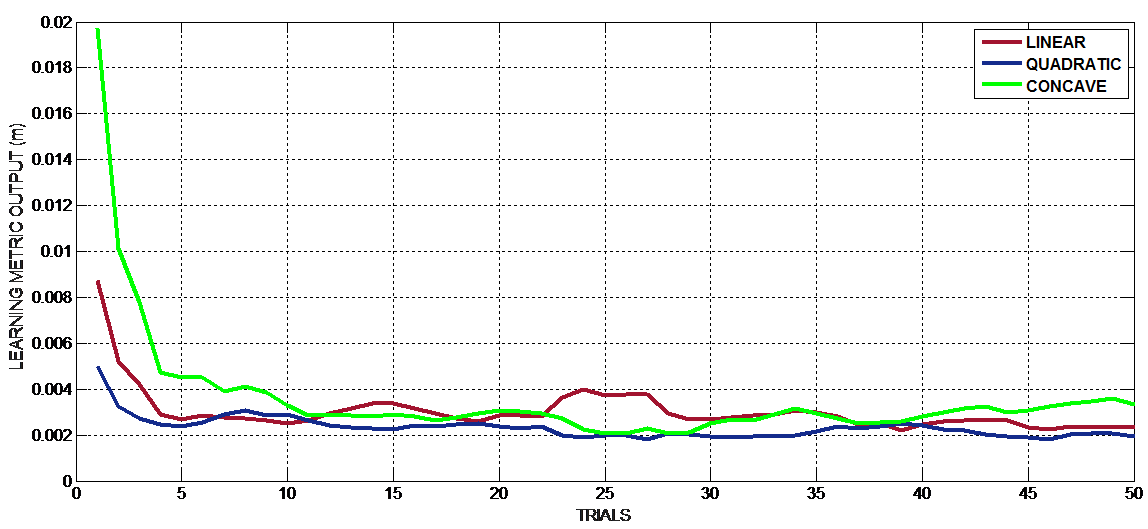
\includegraphics[scale=0.5]{Chie/figs/Figure12.png}
  \caption{Averaged learning performance of the 18 participants over 50 trials in the learning phase of three different forces.}
  \label{learning}
\end{figure}
Figure 13 illustrates the standard error observed in each trial. The deviation of the learning metric value does not vary much especially in case of quadratic force. However, in both linear and concave forces the deviation seems to be varying depend on the number of trials or repetitions. This could be a result of the speed in reaching the target position or fatigue.
%
\begin{figure}
  \centering
  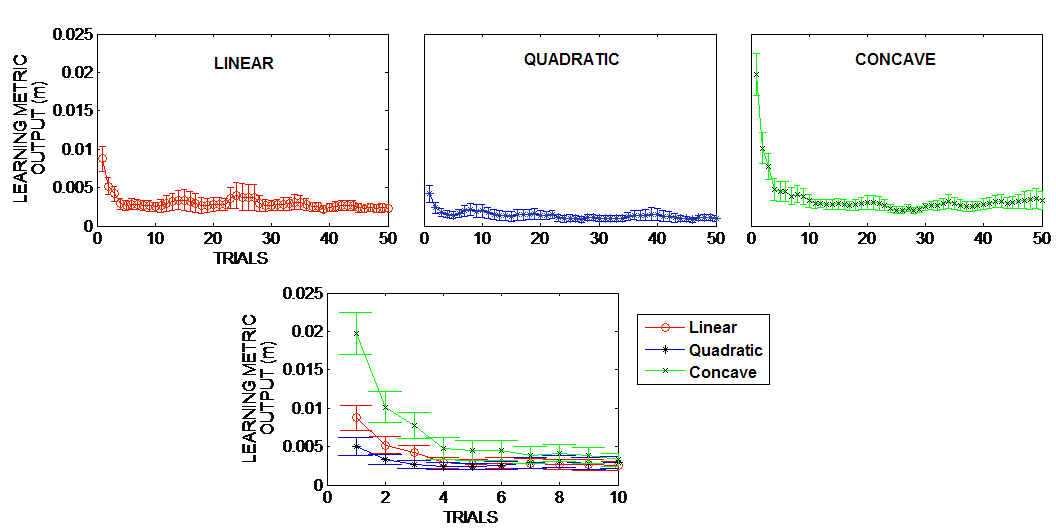
\includegraphics[scale=0.5]{Chie/figs/Figure13.png}
  \caption{ Learning performance of the 18 participants along with the standard error. A big variation in the learning performance of the three different forces is observed within the initial 10trials.}
  \label{learnerror}
\end{figure}
Metric evaluation results of the learning performance of  participants,
\begin{enumerate} 

1.	Concave force seems to be more un-natural, based on the learning curve variance.
 
2.	Linear force has less errors but the learning model maintains a stable condition after n trials, assuming that the learning is good but with the constant overshoots in position. 

3.	Quadratic force seems to be a “well known” force but still the performance gradually improves over the course of trials. The force model helps the user to achieve more precise and accurate movements. 
\end {enumerate}

The time taken to reach the target position or the distance covered is also plotted to understand the specific behaviour of the different learning performance, as shown in Figure 14. All the participants, irrespective of their gender or dominant hand, approached the quadratic force with longer time and being more considerate in reaching the target position. In case of linear and concave model the participants tend to approach the target more rapidly which again resulted in the lack of judgement in being more precise and not learning to reach the target position accurately. Since both the linear and concave model had an increased contact force at the initial stages it can be a result of the same in reaching the target.
%
\begin{figure}
  \centering
  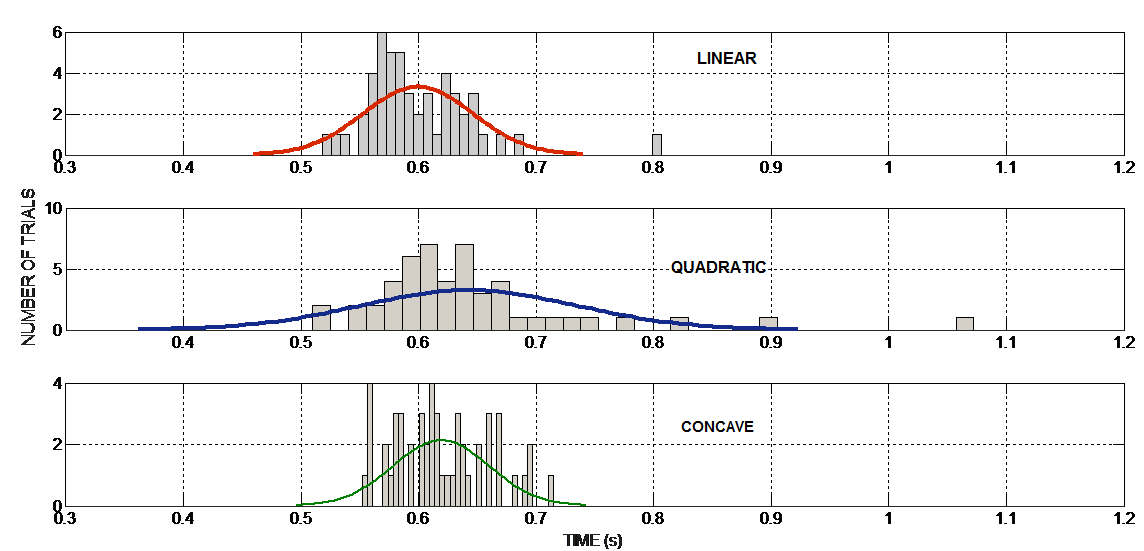
\includegraphics[scale=0.5]{Chie/figs/Figure14.png}
  \caption{Average Time taken by the 18 participants to reach the target Z=0.12m with the three different forces }
  \label{speed}
\end{figure}
The Probability distribution of the time for different force models are presented here, 
\begin{enumerate}

1.	Quadratic force model is very fragile but still the time reaching the target is quite wide range

2.	Both Concave and Linear have a similar behaviour in terms reachable time. 

3.	Although the initial force is high in concave model the time taken to reach the target is quite low- which will explain the higher over shoots. 
\end{enumerate}

This time also explains the learning capability of the force dynamics, lower force takes longer time than the higher force.

\subsubsection{Questionnaires}
The responses for both the questions can be shown in Table 3 and Figure 15. The Table provide individual responses with their demographic information and the two bar charts illustrate the averaged data across 18 participants.

The Table 3 showed that majority of the participants $(55.5\%)$ could not differentiate between linear and non-linear forces.  $44.5 \% $of the participants succeeded in identifying the difference between a linear and non-linear accurately.
begin{figure}
  \centering
  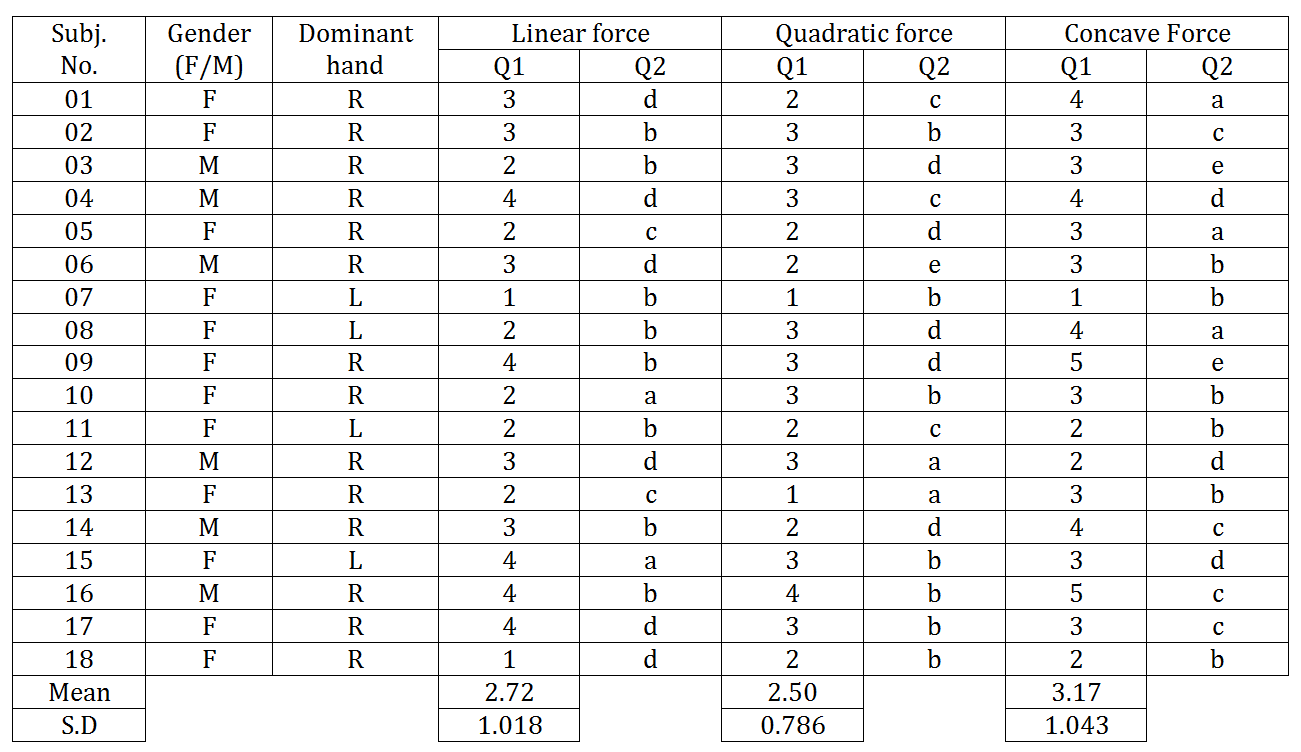
\includegraphics[scale=0.4]{Chie/figs/Table3.png}
  \caption{Participant demographic information and the questionnaire responses}
  \label{Table1}
\end{figure}

According to the Figure 15, participants rated more effort on to the Concave force after the session.
A statistical analysis was made for the results of the Q1. Mauchly’s test of Sphericity indicated that the assumption of sphericity had not been violated, $χ^2 (2) = 0.287, p = .866$. A repeated measures ANOVA showed that mean effort differed significantly between three type of forces,$ F(2,34) = 5.633, p = .008 < .05$. Post hoc tests using the Bonferroni correction revealed that the mean difference was only significantly between the Quadratic and the Concave (p = .019).
%
\begin{figure}
  \centering
  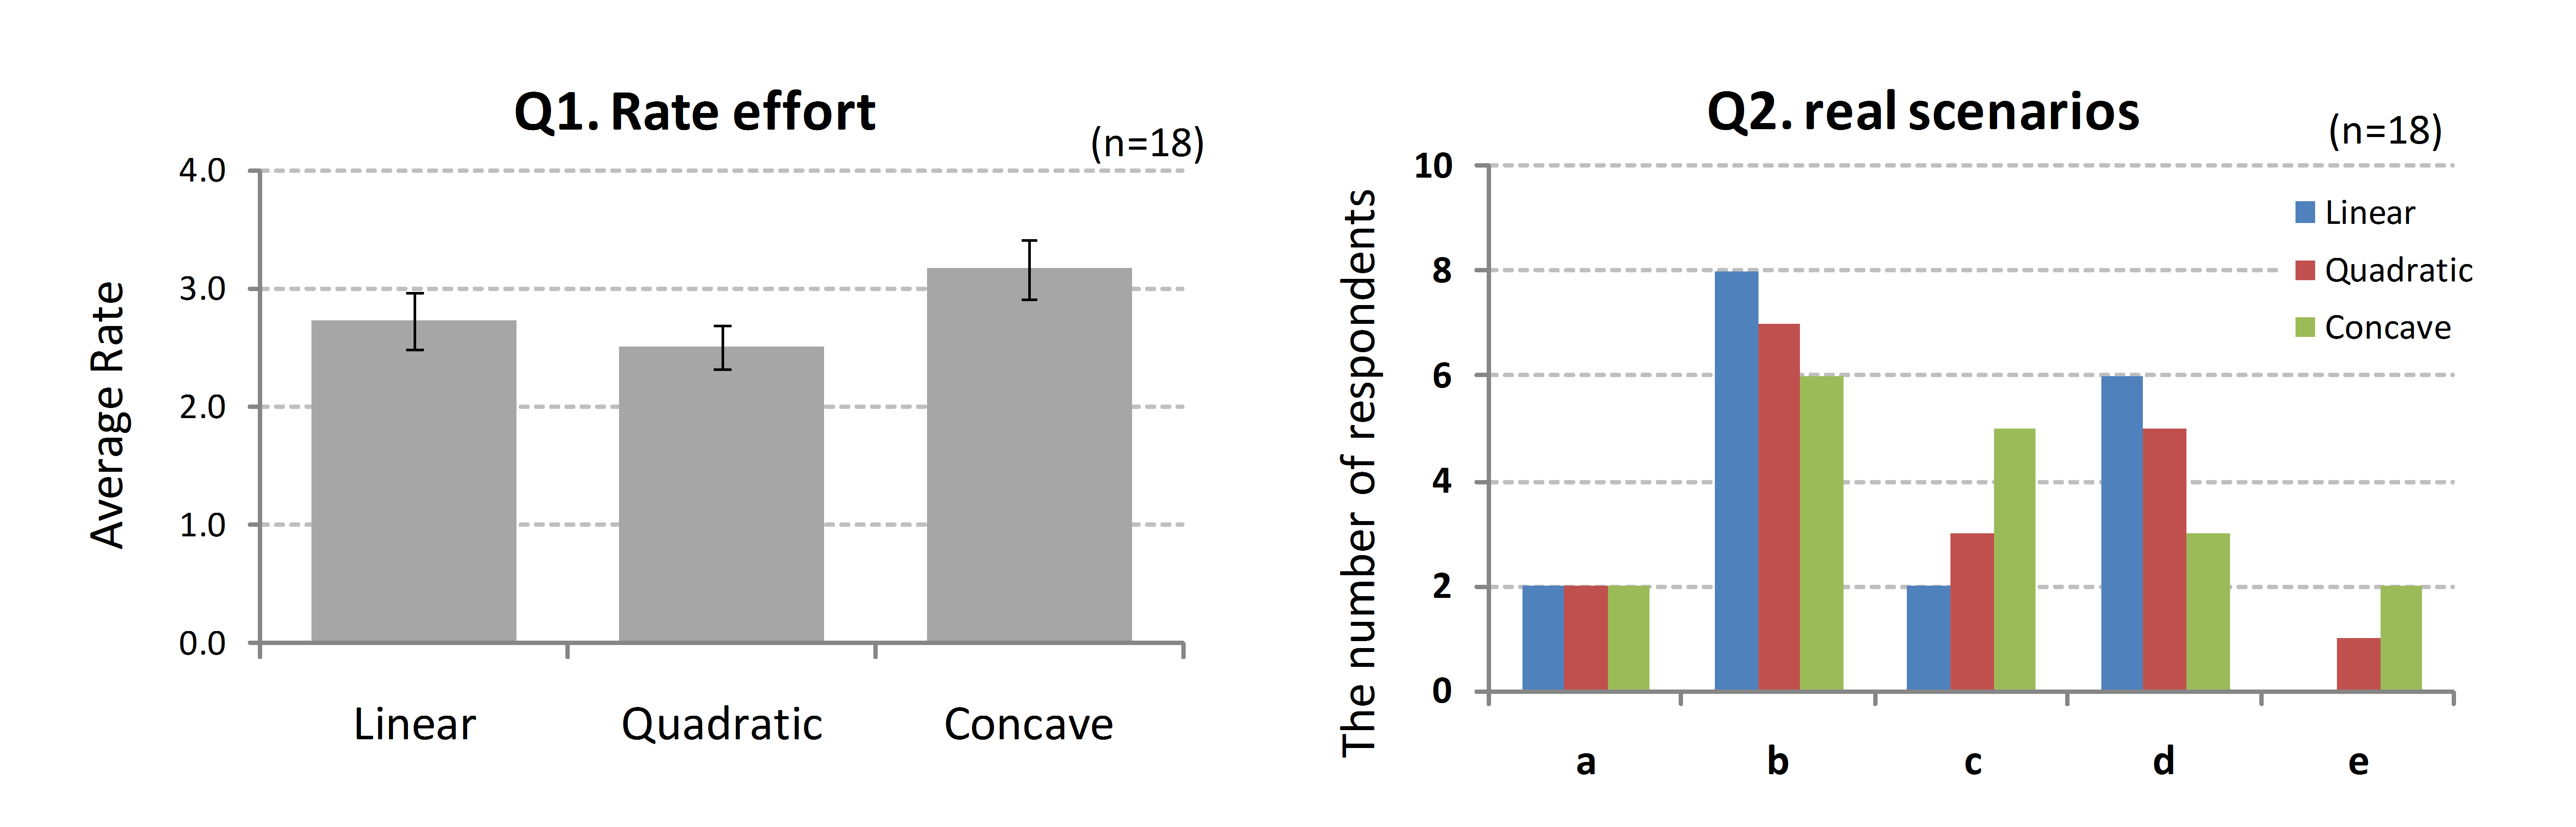
\includegraphics[scale=0.5]{Chie/figs/Figure15.png}
  \caption{Q1. Average rate of the effort for three different forces across 18 participants. Q2. The number of respondents considering five real scenarios: a. cushion, b. revolving door, c. box on a plane surface, d. hinged door, e. a box on an inclined surface.  See more details at the Method section. }
  \label{questionnaire}
\end{figure}
It is hard to analyse the results of the Q2: real scenarios, and to examine the correlation between the Q1 and Q2. The number of participants was only 18, and their individual differences on the force perception seemed to be larger than their differentiation among three types of forces. Also, their force perception might have strongly affected by the task itself rather than the force type itself. Even though there were difficulties to interpret the responses, the Q2 bar graph indicated that some pattern clearly existed among three forces. There are possible ways to make further analyses; for example, to increase the number of participants and to evaluate the perception differences from their normalised (baseline) performance. This is a challenging research theme but very important in this research area. Further analysis should be made to bridge between physical properties and subjective human force perception.







